\section{Experiments}


\subsection{MONK's results}

The neural networks used for the problems have 17 input units, the number of hidden units are written in table \ref{tab:dati}  and the output layer has always one unit. We used \texttt{tanh} as a hidden layer activation function and \texttt{sigmoid} as an output layer activation function. We chose \texttt{Mean squared error} as the loss function. An input is classified as 1 if the output of the neural network is greater than 0.5 or 0 otherwise.\\
We used stochastic, mini-batch and batch gradient descent but in the end we decided to use the batch gradient descent because loss function plots were smoother than the others.
We also used the weight decay regularization as the lambda parameter and Nesterov momentum as the momentum parameter. Table \ref{tab:dati} reports the average of the values found for TR and TS after five different trainings of the networks. For the training phase we initialized the weight with a uniform distribution in the interval [-1e-3, 1e-3].    
\begin{center}
\small\addtolength{\tabcolsep}{-5pt}
\begin{table}[H]
\begin{tabular}{|c|c|c|c|c|c|c|}
\hline
\textbf{Task} &	\textbf{\#Units} &\textbf{ eta} & \textbf{lambda} &\textbf{momentum} & {\textbf{MSE(TR/TS)}} &\textbf{Accuracy(TR/TS)} \\ \hline
MONK 1        &    3 & 0.9 & 0 & 0.7  &   6.3e-4/1e-3 &   100\%/100\%  \\ \hline
MONK 2        &    4 & 0.8 & 0 & 0.7  &   1e-3/1.3e-3 &   100\%/100\% \\ \hline               
MONK 3        &    5 & 0.4 &5e-3 &0.2&     7.8e-2/5.5e-2&    93.44\%/97.22\%  \\ \hline
MONK 3 (no reg)&   5 & 0.6 &   0 &  0.7 &   1.7e-2/2.7e-2 & 95.90\%/93.51\%		\\ \hline              
\end{tabular}
\caption{MONK's problems parameter and results.}
\label{tab:dati}
\end{table}
\end{center}
\subsubsection{MONK 1}

\begin{figure}[H]
    \centering
    \begin{minipage}[t]{0.5\linewidth}
        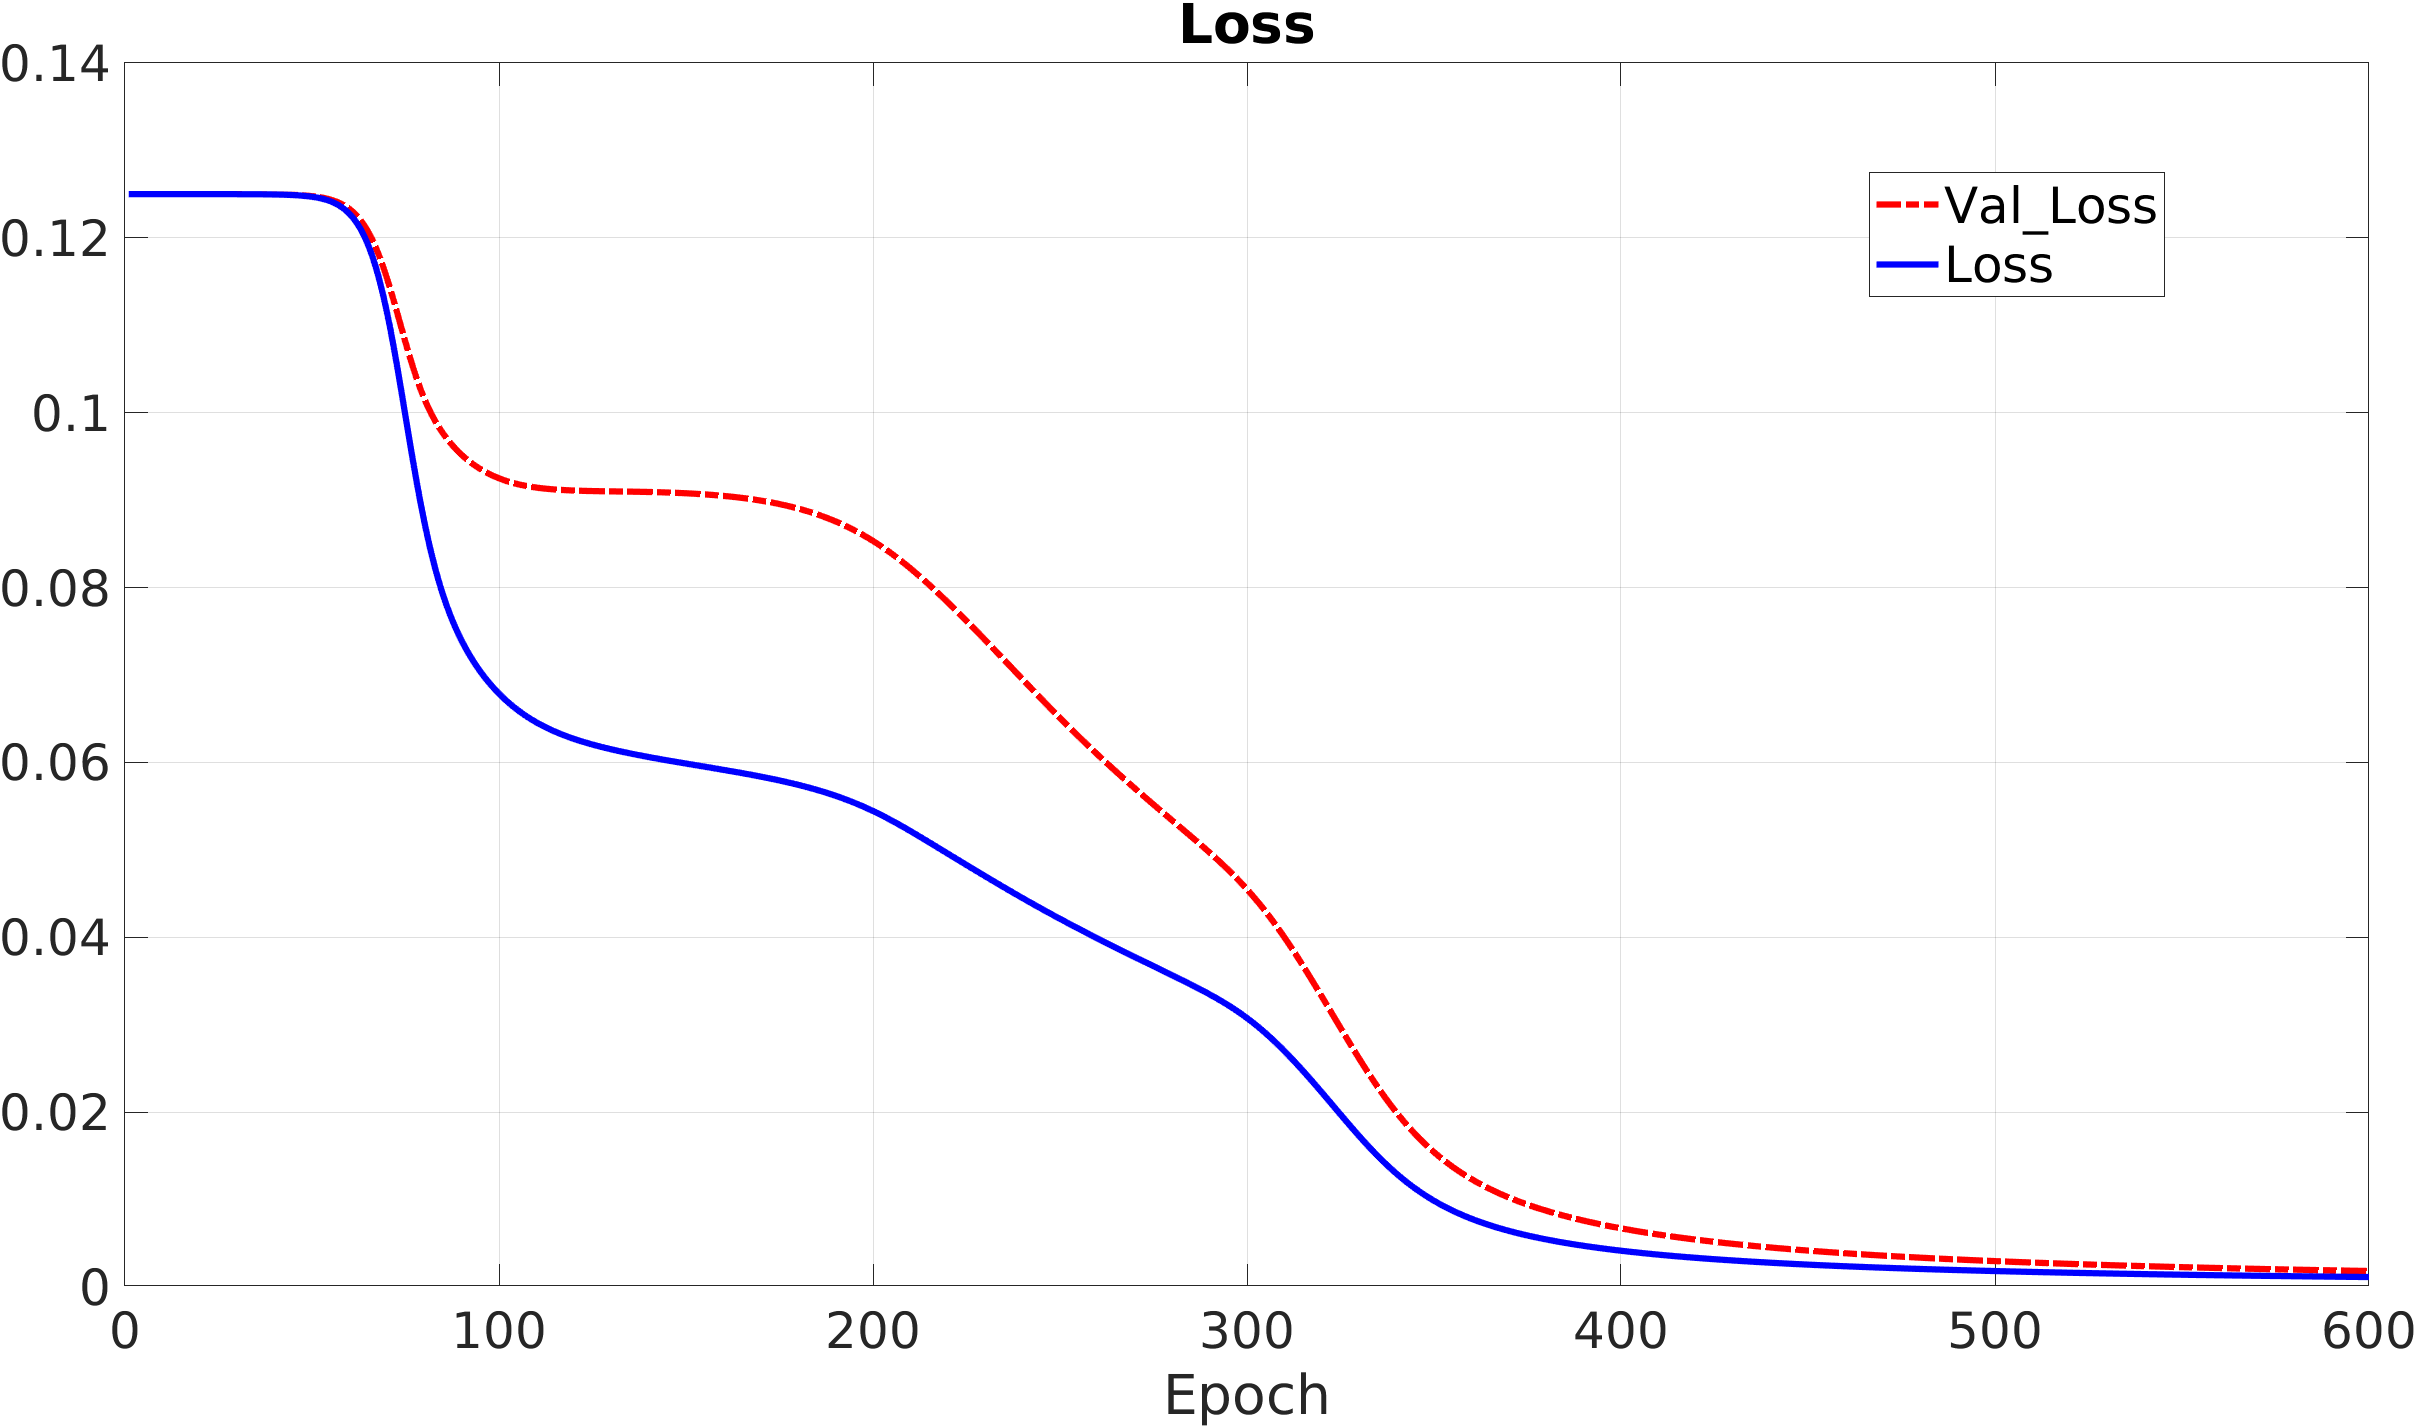
\includegraphics[width=\linewidth]{img/Monk1_loss.png}
        %\subcaption{MSE}
    \end{minipage}%
    \begin{minipage}[t]{0.5\linewidth}
        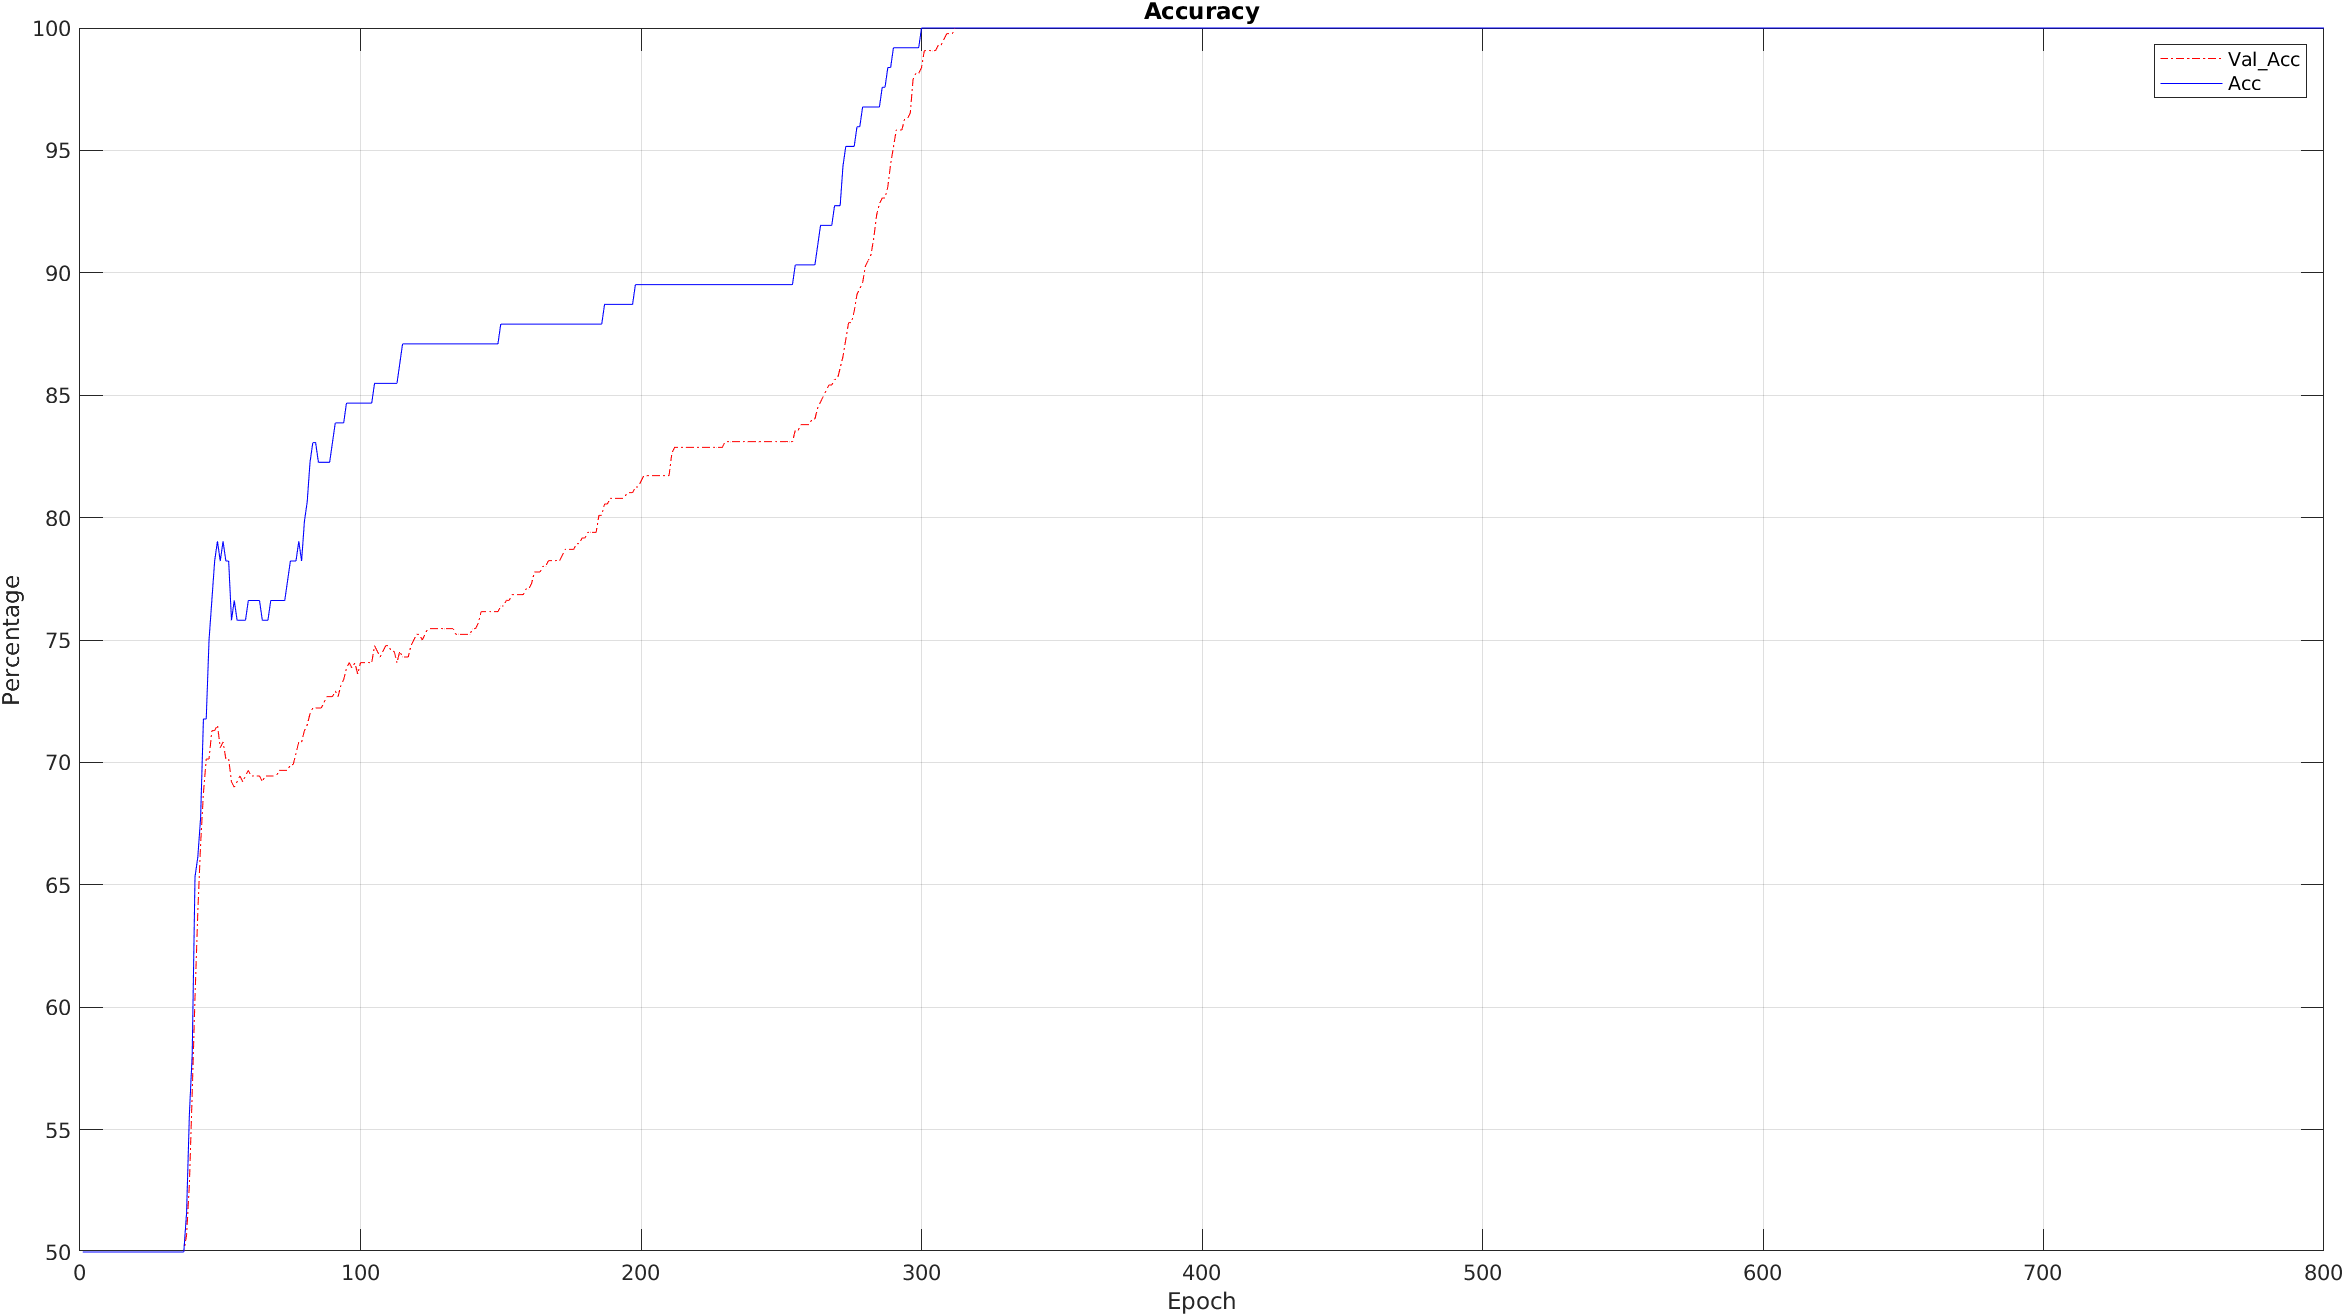
\includegraphics[width=\linewidth]{img/Monk1_accuracy.png}
        %\subcaption{Accuracy}
    \end{minipage}
    \caption{MSE and accuracy for MONK’s 1.}
\end{figure}

\subsubsection{MONK 2}
\begin{figure}[H]
    \centering
    \begin{minipage}[t]{0.5\linewidth}
        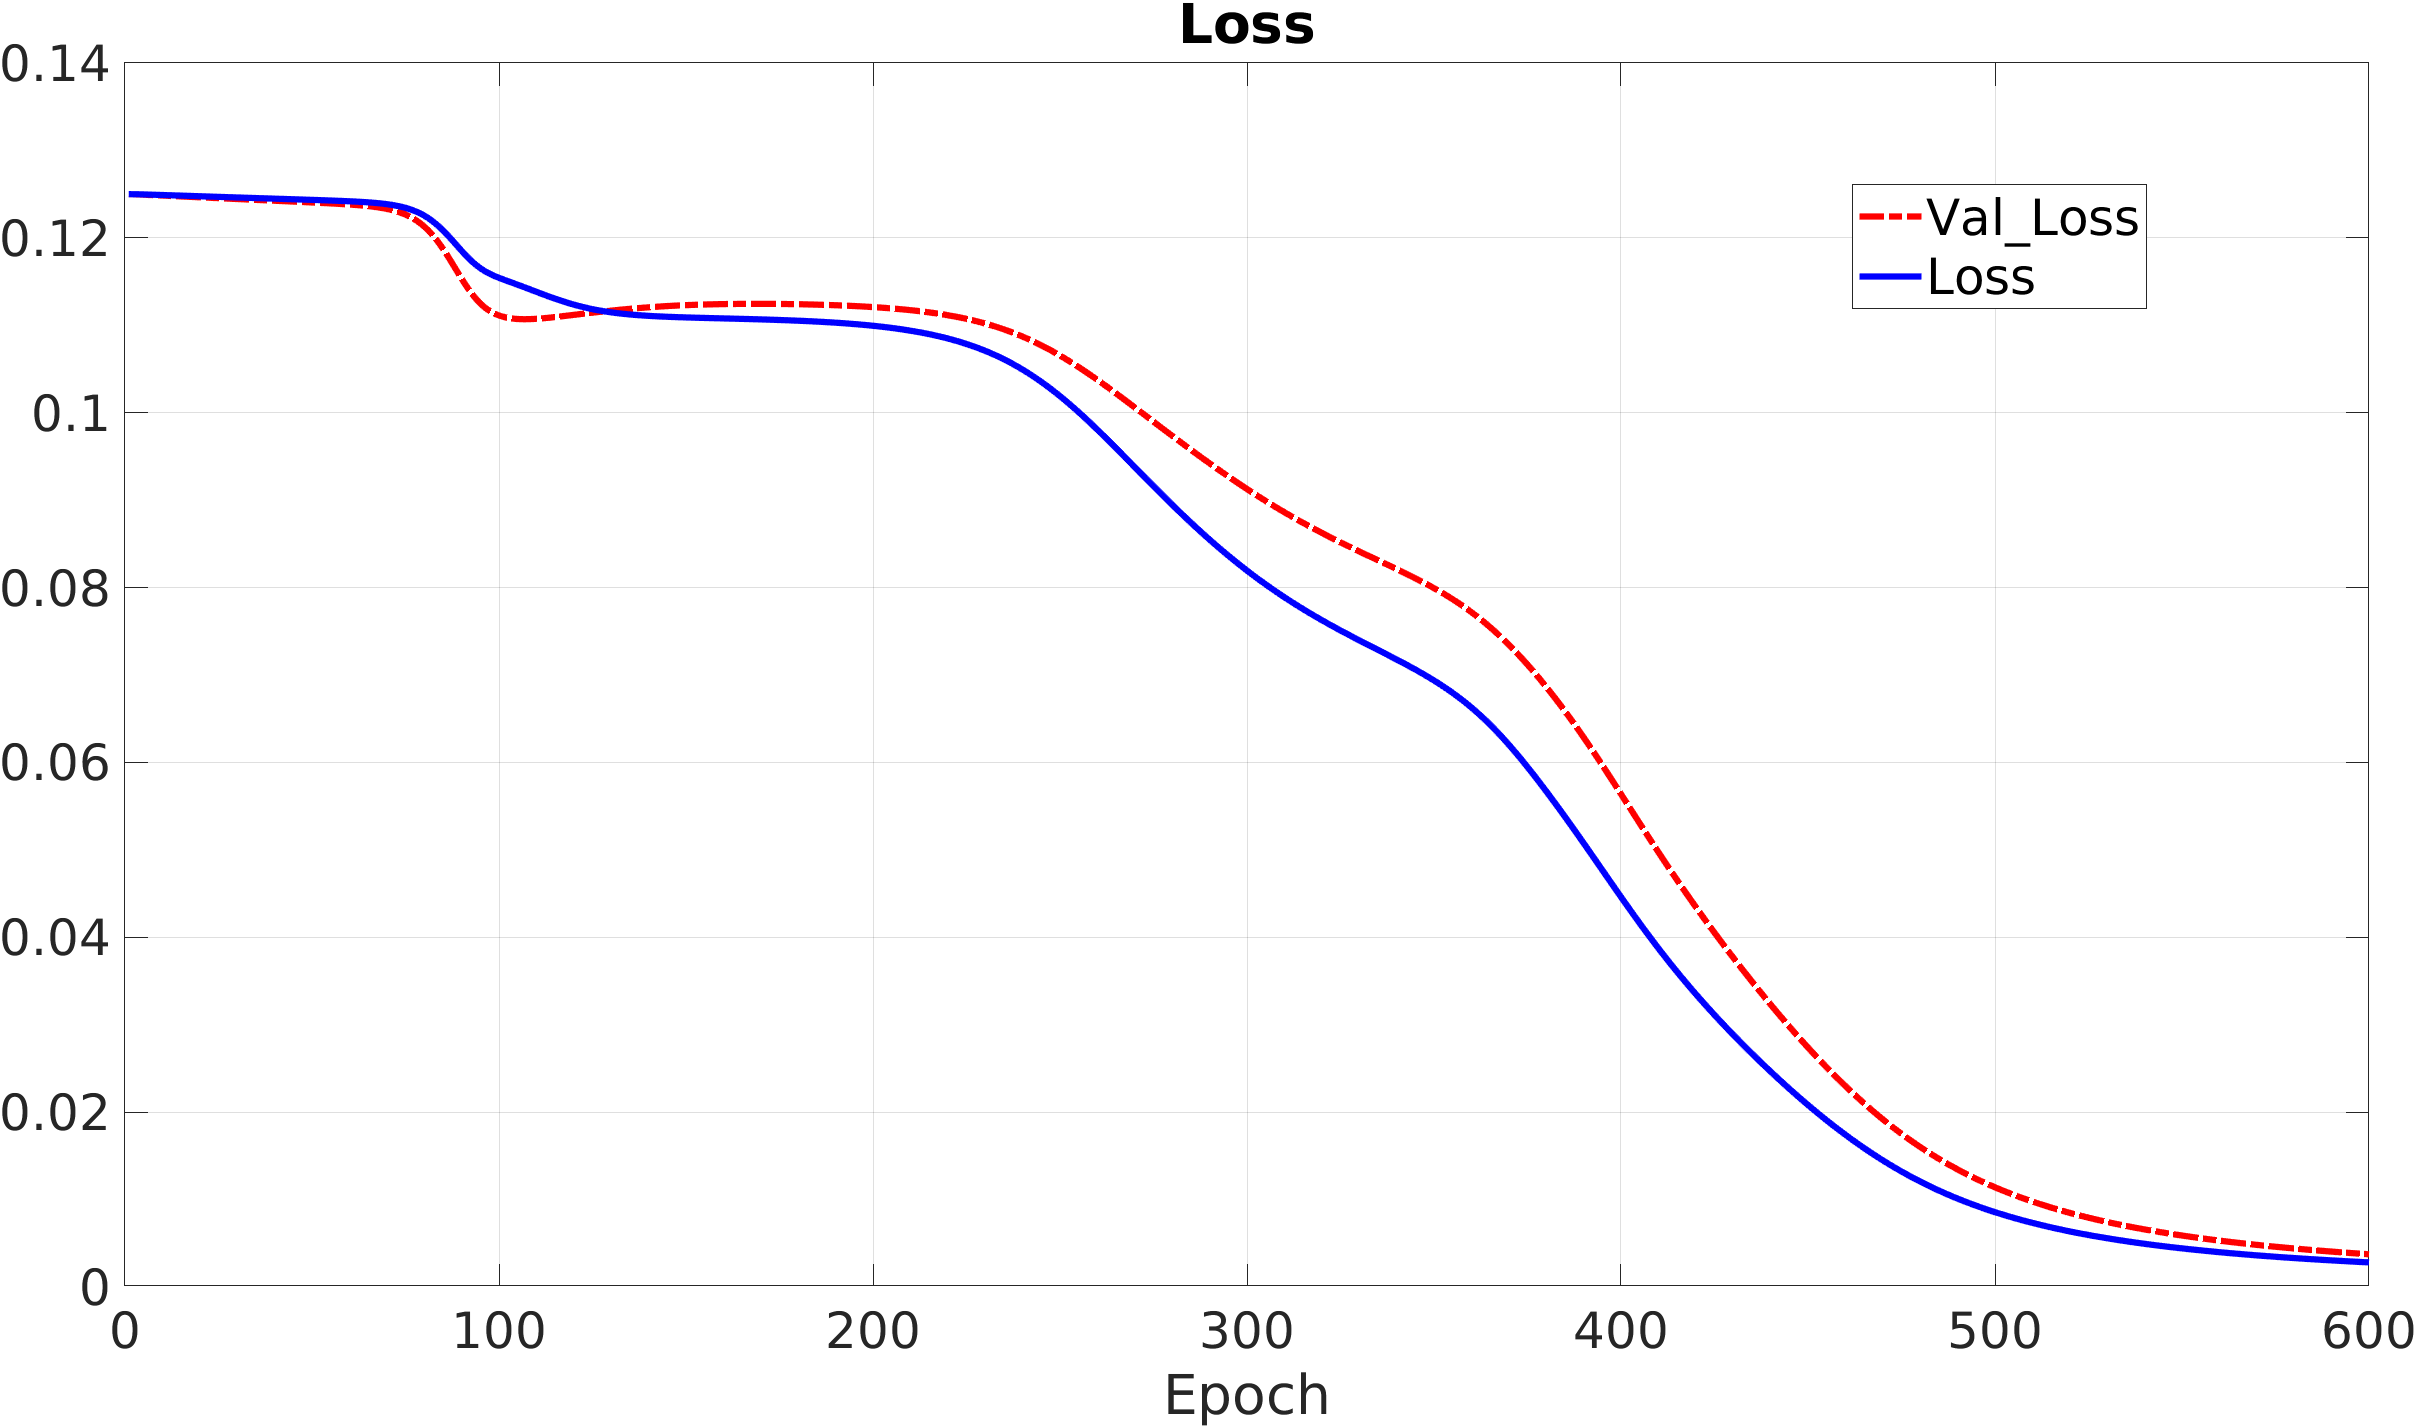
\includegraphics[width=\linewidth]{img/Monk2_loss.png}
        %\subcaption{MSE}
    \end{minipage}%
    \begin{minipage}[t]{0.5\linewidth}
        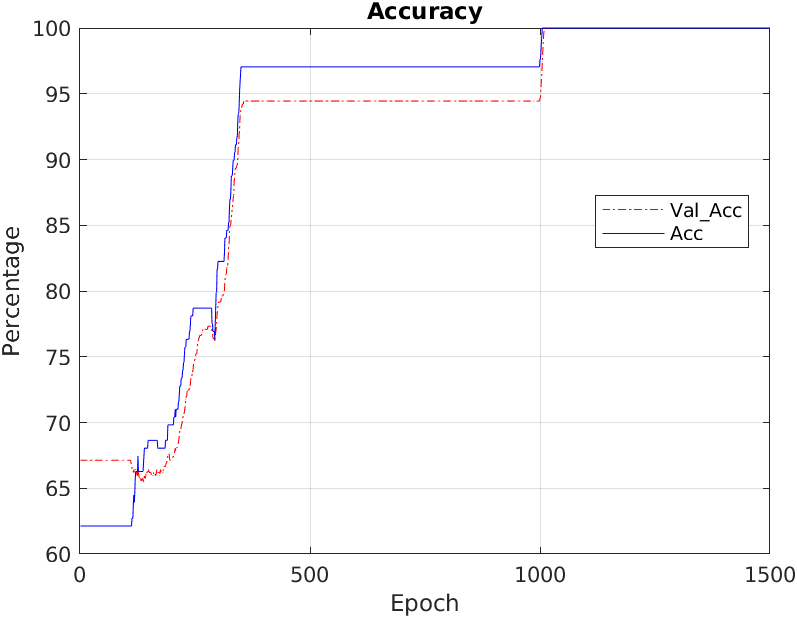
\includegraphics[width=\linewidth]{img/Monk2_accuracy.png}
        %\subcaption{Accuracy}
    \end{minipage}
    \caption{MSE and accuracy for MONK’s 2.}
\end{figure}

\subsubsection{MONK 3}
We figured out during the training phase that the learning curves of MONK's 3 without regularization showed overfitting in the output (see fig. \ref{fig:m3nr}). In response to that, we fixed it by adding regularization. We obtained better results since the training didn't show overfitting in the validation error (see fig. \ref{fig:m3r}).
\begin{figure}[H]
    \centering
    \begin{minipage}[t]{0.5\linewidth}
        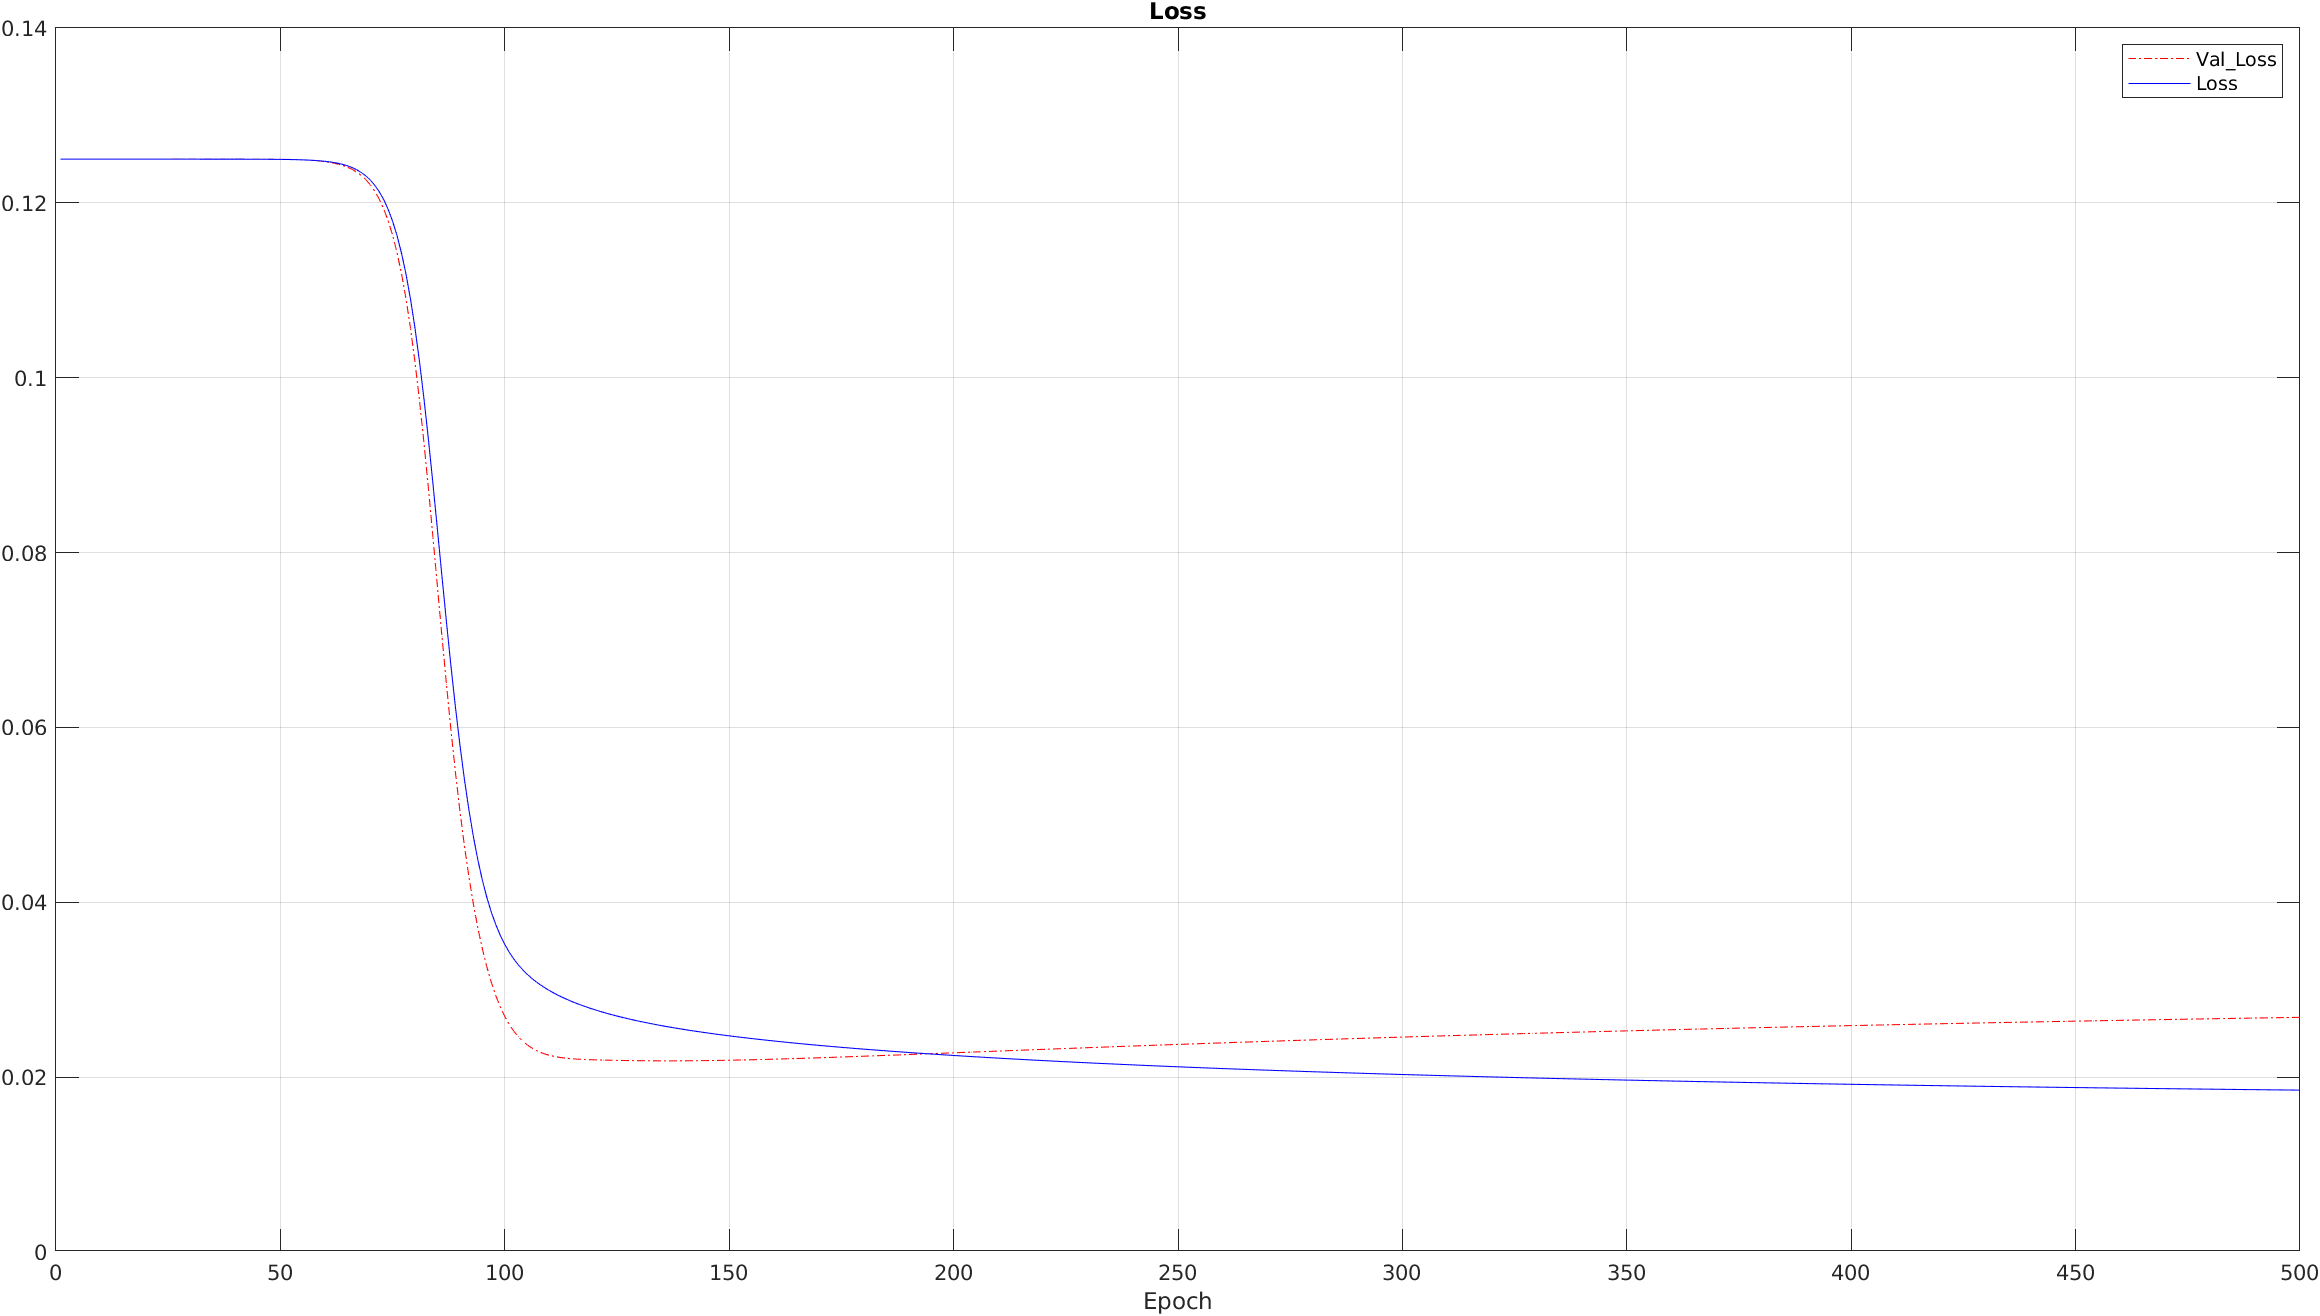
\includegraphics[width=\linewidth]{img/Monk3_loss_noReg.png}
        %\subcaption{MSE}

    \end{minipage}%
    \begin{minipage}[t]{0.5\linewidth}
        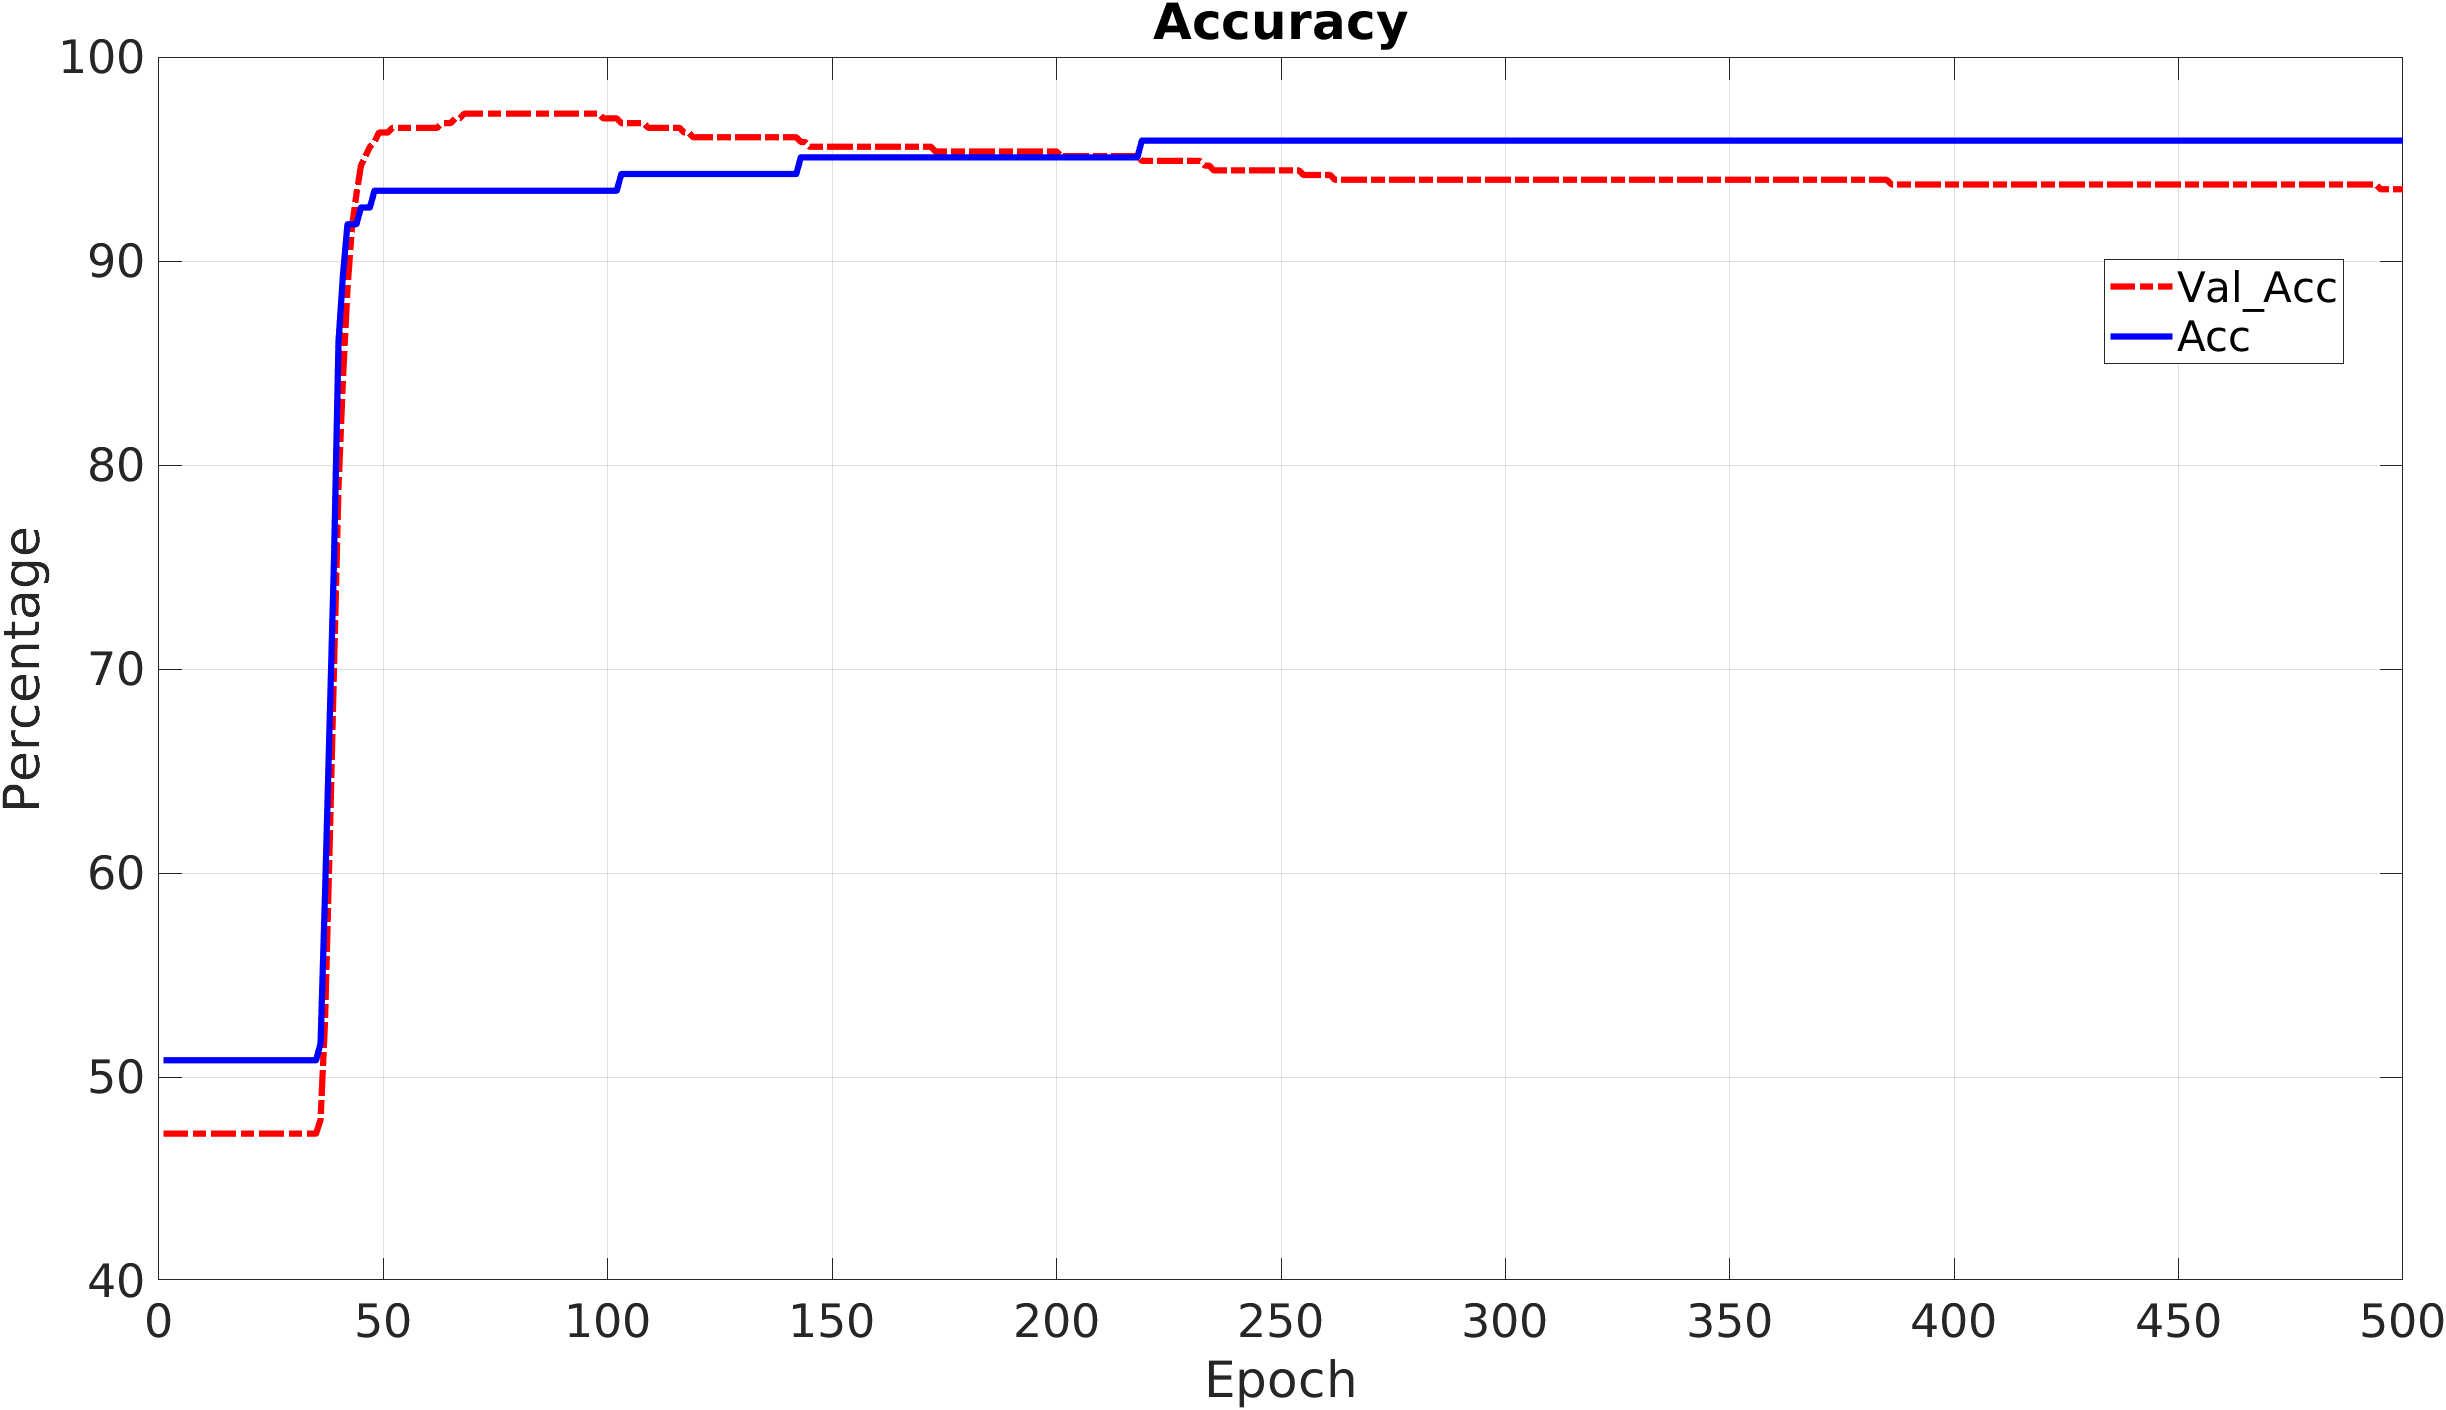
\includegraphics[width=\linewidth]{img/Monk3_accuracy_noReg.png}
        %\subcaption{Accuracy}
    \end{minipage}
    \caption{MSE and accuracy for MONK’s 3 not regularized.}
    \label{fig:m3nr}
\end{figure}

\begin{figure}[H]
    \centering
    \begin{minipage}[t]{0.5\linewidth}
        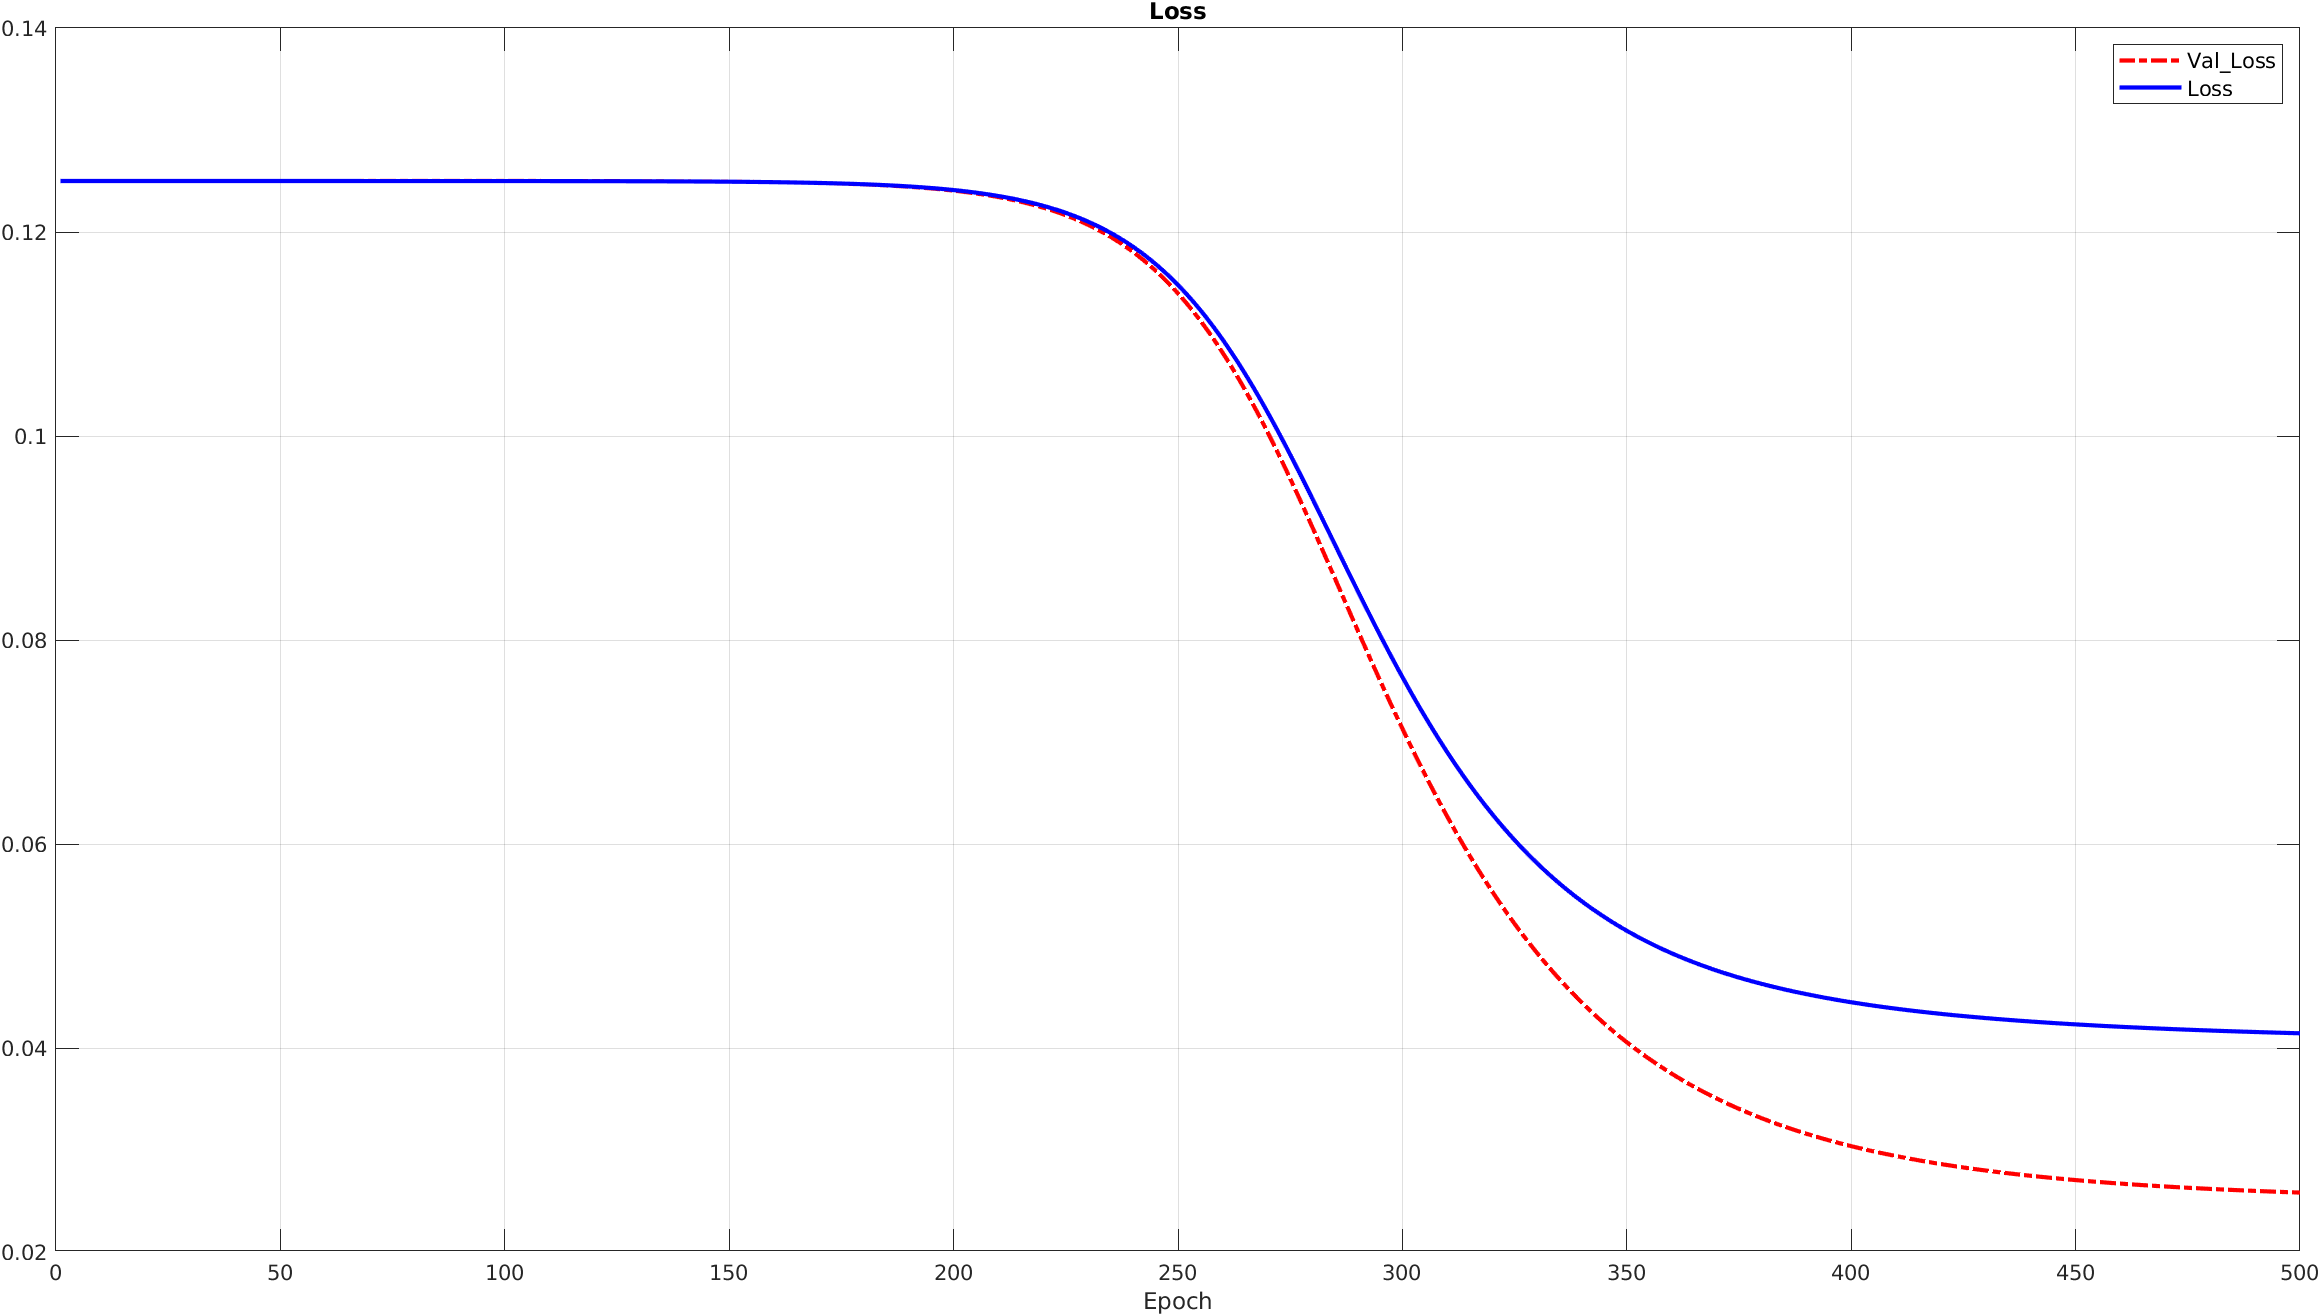
\includegraphics[width=\linewidth]{img/Monk3_loss_Reg.png}
        %\subcaption{MSE}
    \end{minipage}%
    \begin{minipage}[t]{0.5\linewidth}
        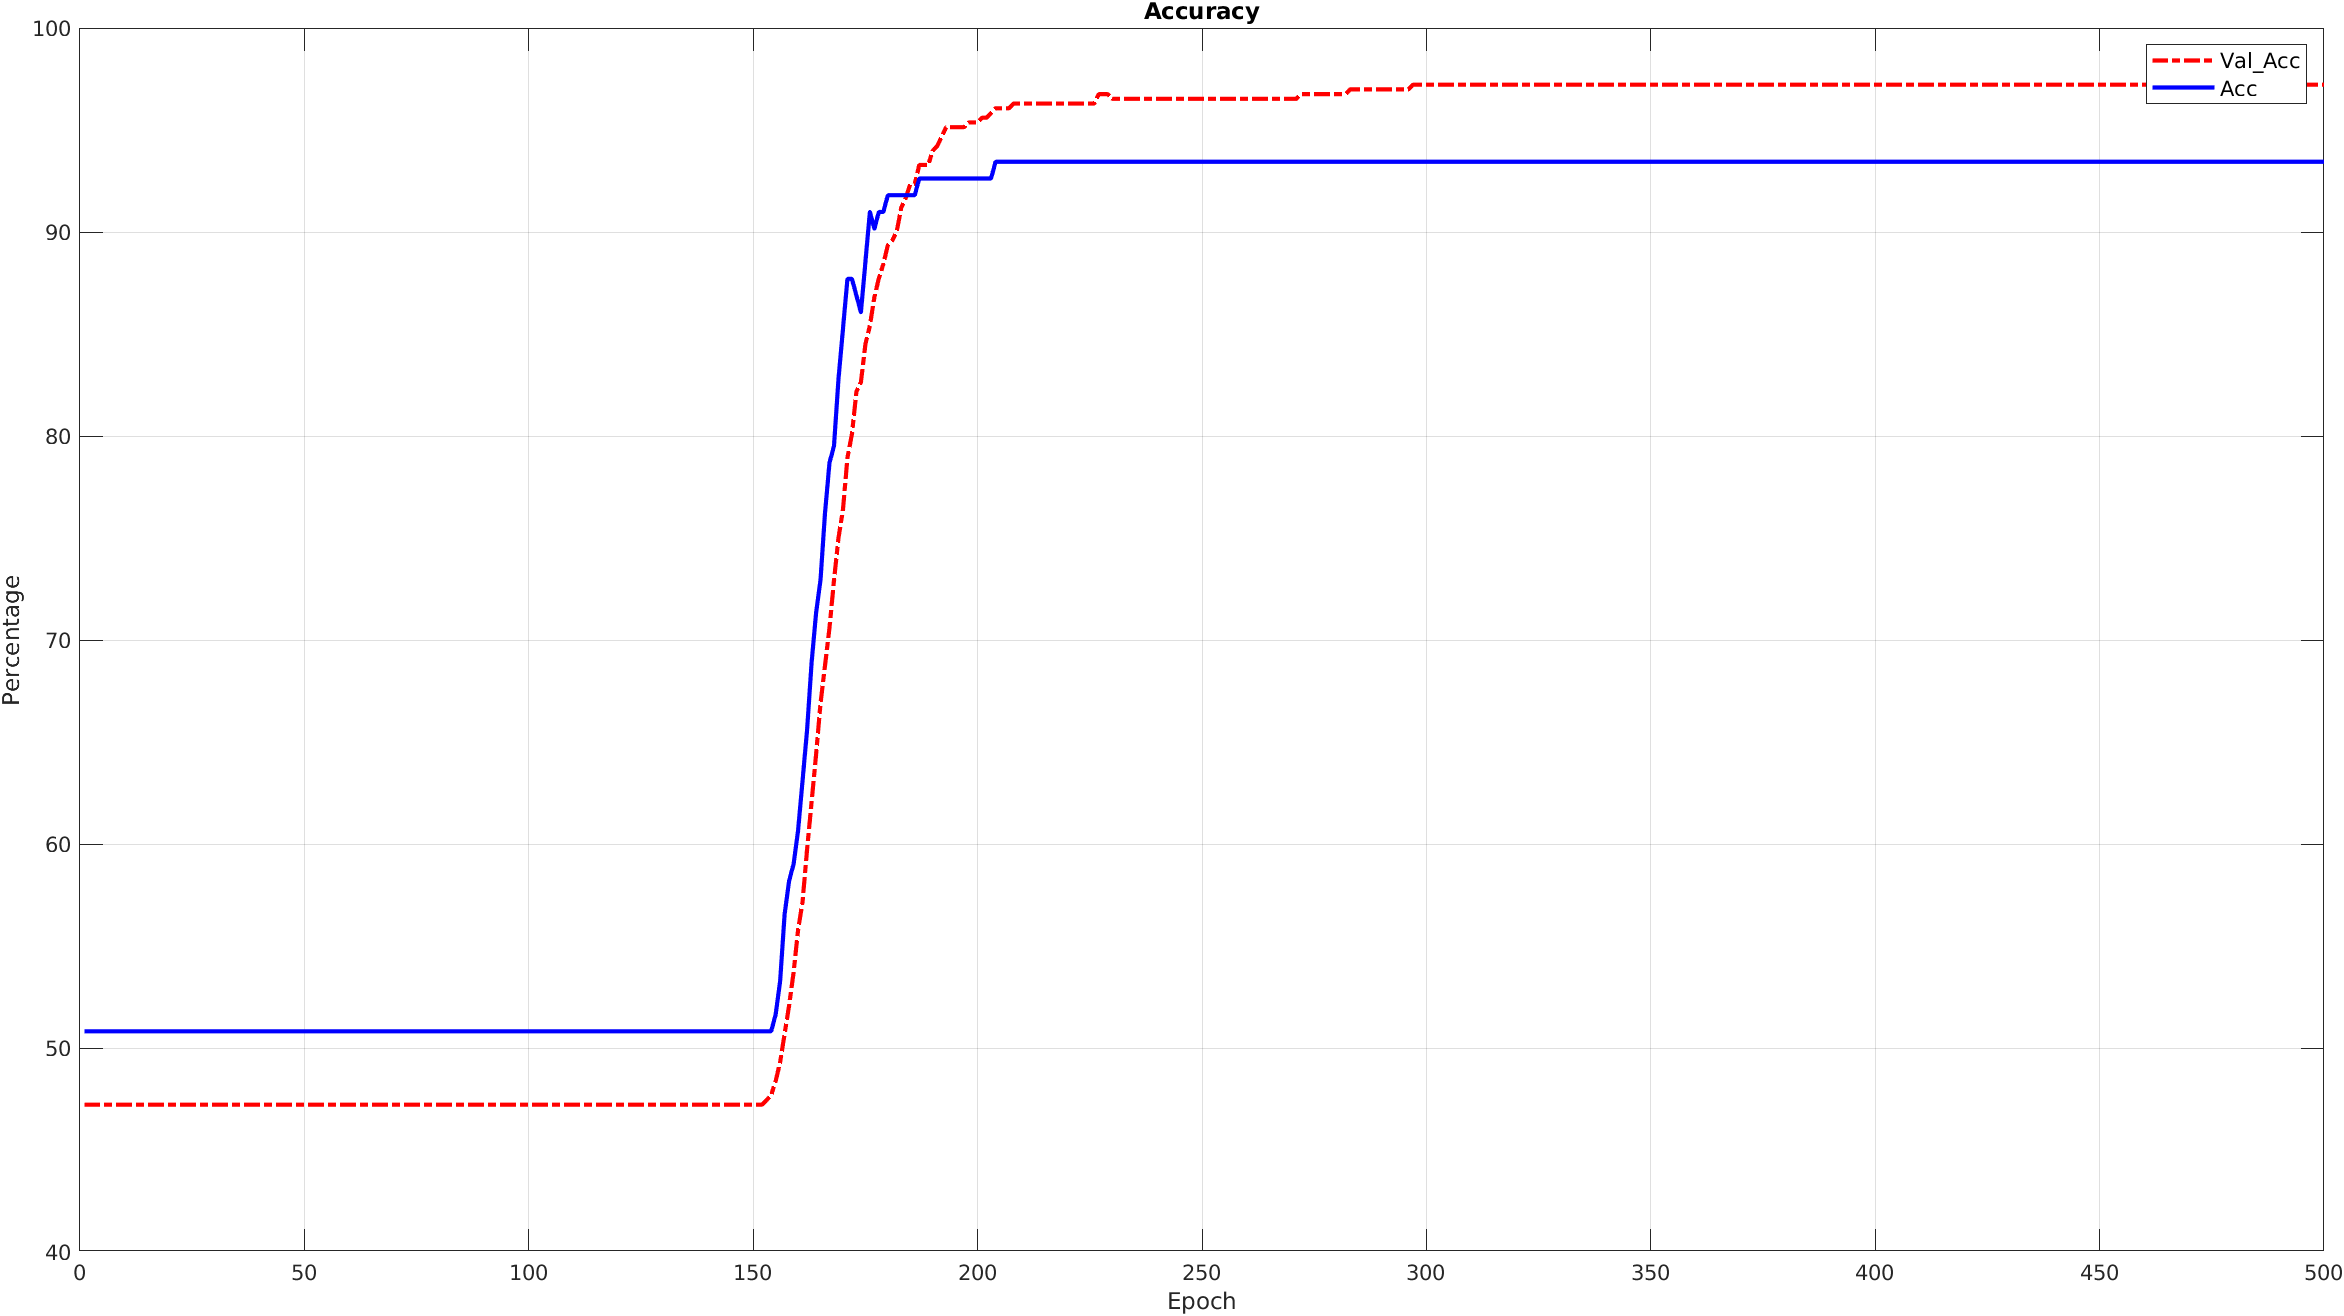
\includegraphics[width=\linewidth]{img/Monk3_accuracy_Reg.png}
        %\subcaption{Accuracy}
    \end{minipage}
    \caption{MSE and accuracy for MONK’s 3 regularized.}
    \label{fig:m3r}
\end{figure}



\subsection{Cup results}

\subsubsection{Validation schema}
Initially, we split the dataset in training set and test set with 80\% (1412 records) for training and 20\% (353 records) for the test. For the selection of the best model, we decided to use k-fold cross validation with k=3. In the end, we chose the best models among all the models trained during the grid search step. We used stochastic, mini-batch and batch gradient descent and we observed that the batch type had smoother learning curves.

\subsubsection{Screening phase}
Firstly we tried with single hidden layer networks and we could already observe good results. For this reason, we tuned the hyper-parameters for this type of network through grid searches.
Then we chose MEE as the loss function for validation and test set. We trained the network with MSE but we plotted the results with MEE to make them comparable with the learning curves of test and validation set.
Later, we focused on finding some variants of the network with more hidden layers. We tuned the hyper-parameters through grid search.
The screening phase turned out to be fundamental since choosing the right search setting of the hyper-parameters saved us a lot of time. We understood  which hyper-parameters needed to be discarded a priori (e.g. high learning rate fig. \ref{img:hlr} or small mini-batch fig. \ref{img:smb}).

\begin{figure}[H]
	\centering
	\begin{minipage}[t]{0.5\linewidth}
		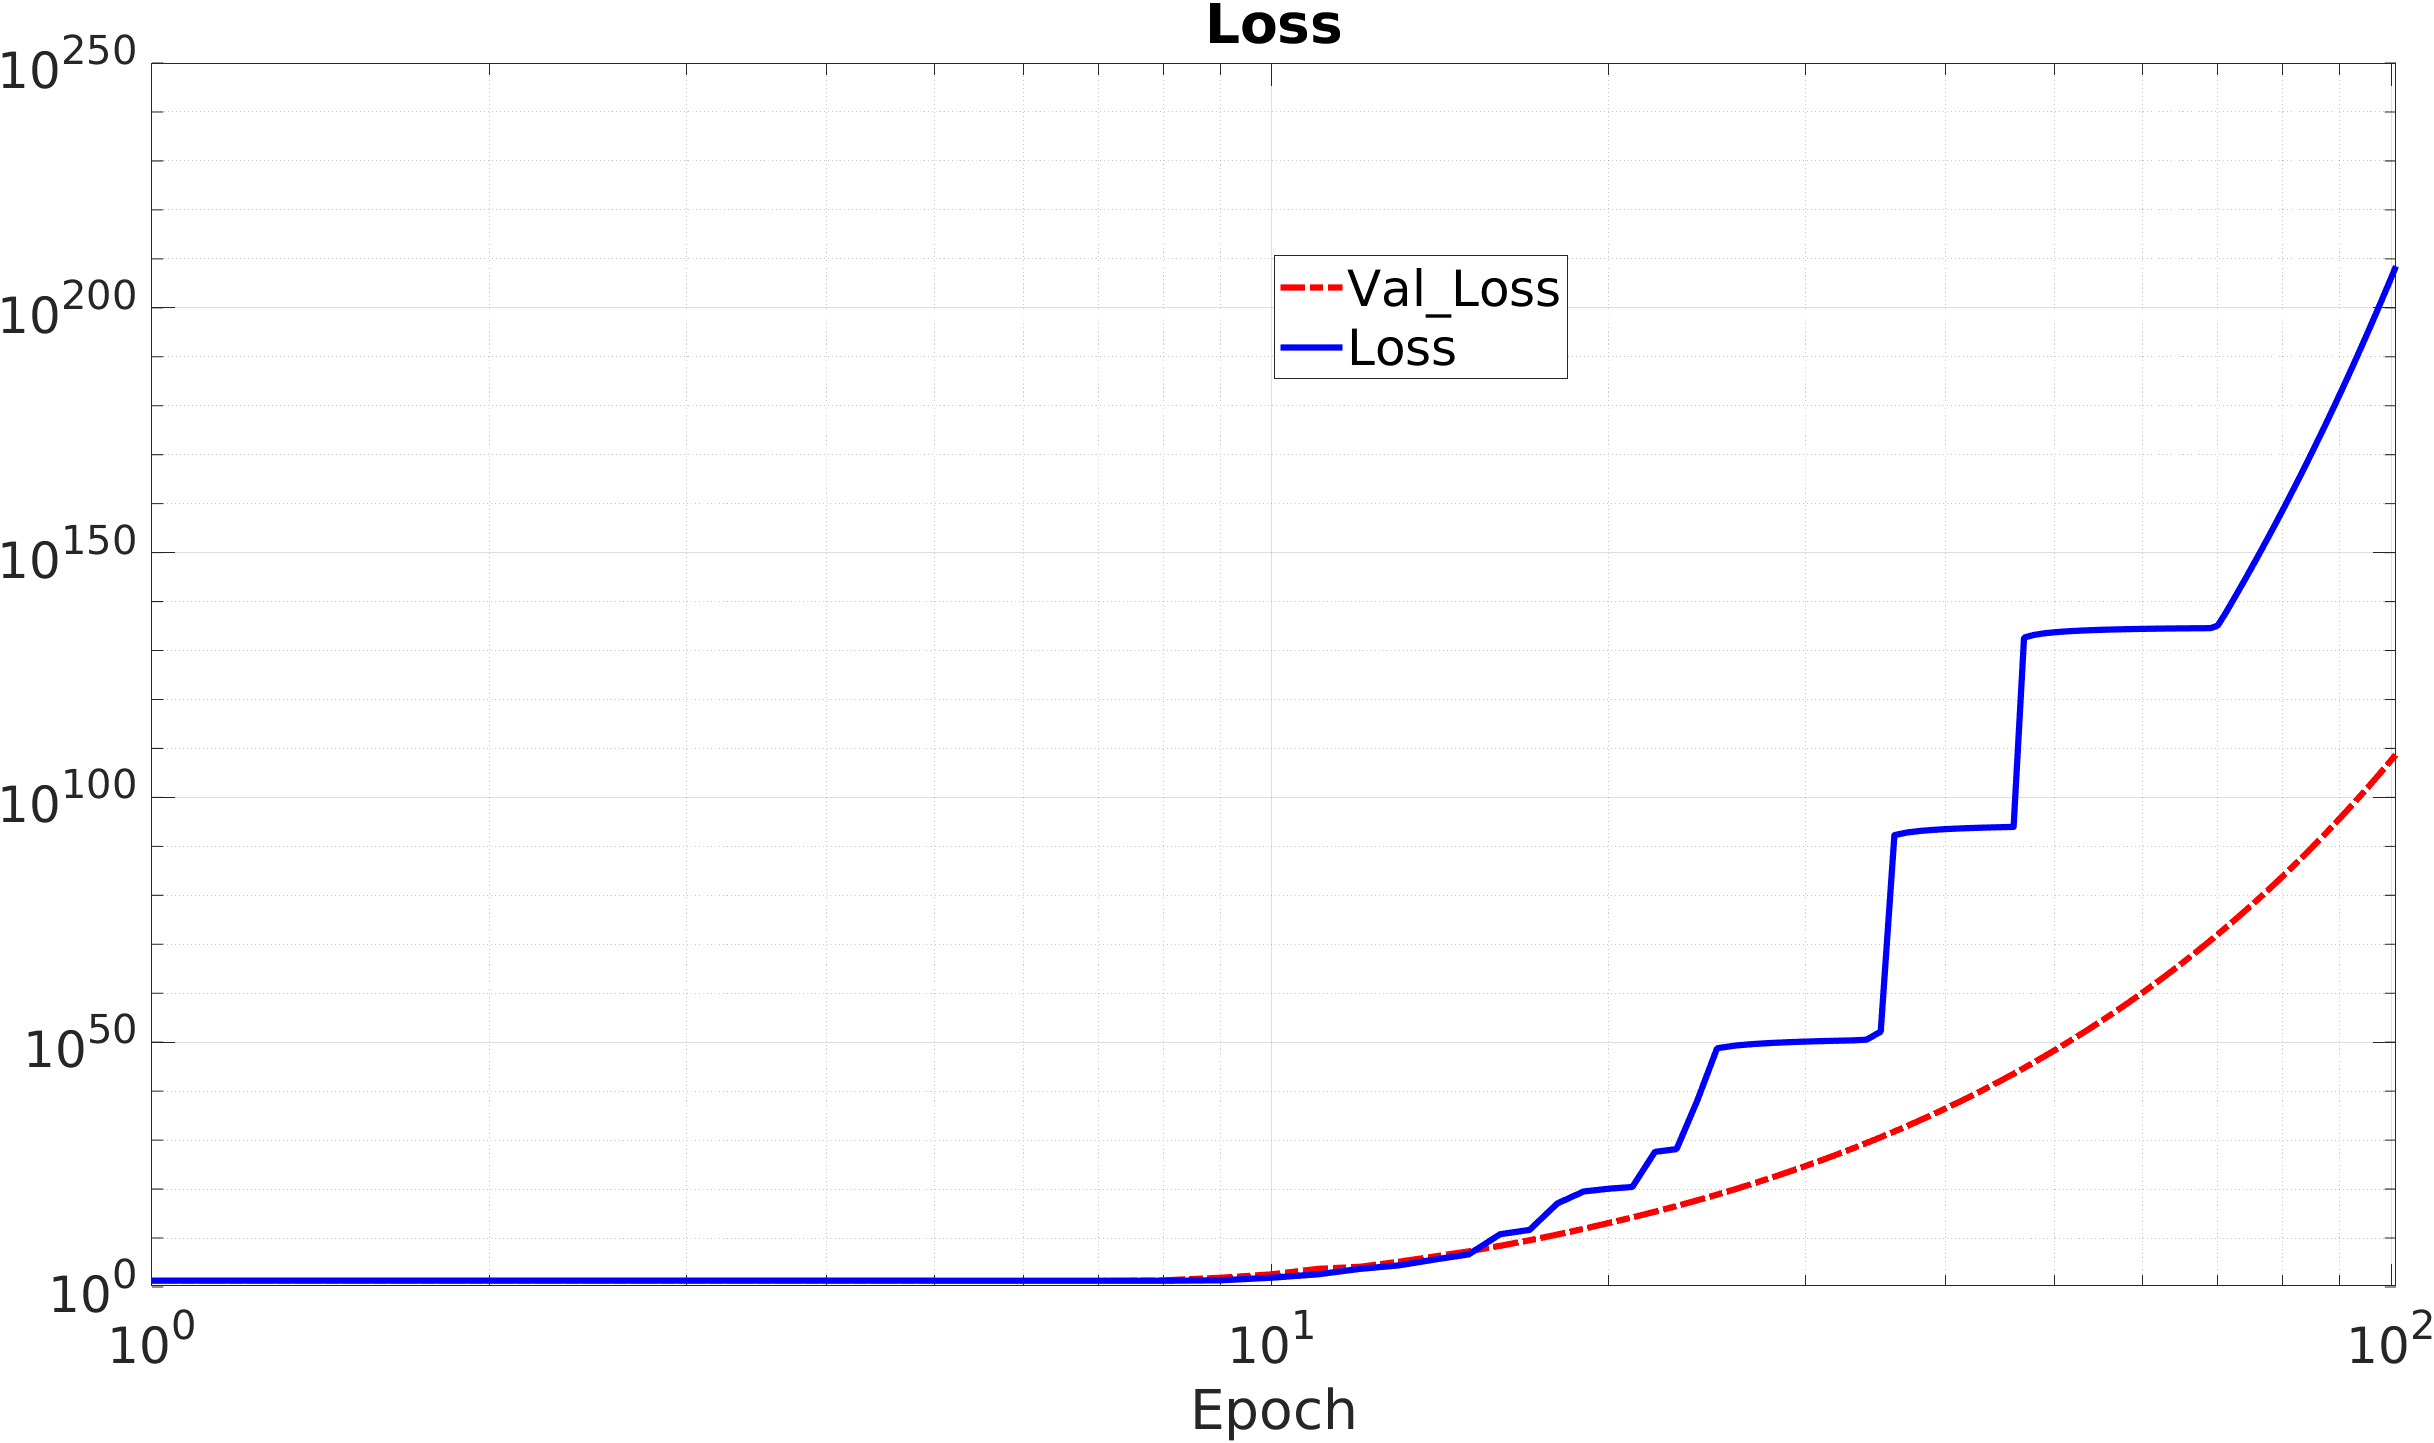
\includegraphics[width=\linewidth]{img/Cup_loss_divergente.png}
		\caption{MEE neural network divergent.}
		\label{img:hlr}
	\end{minipage}%
	\begin{minipage}[t]{0.5\linewidth}
		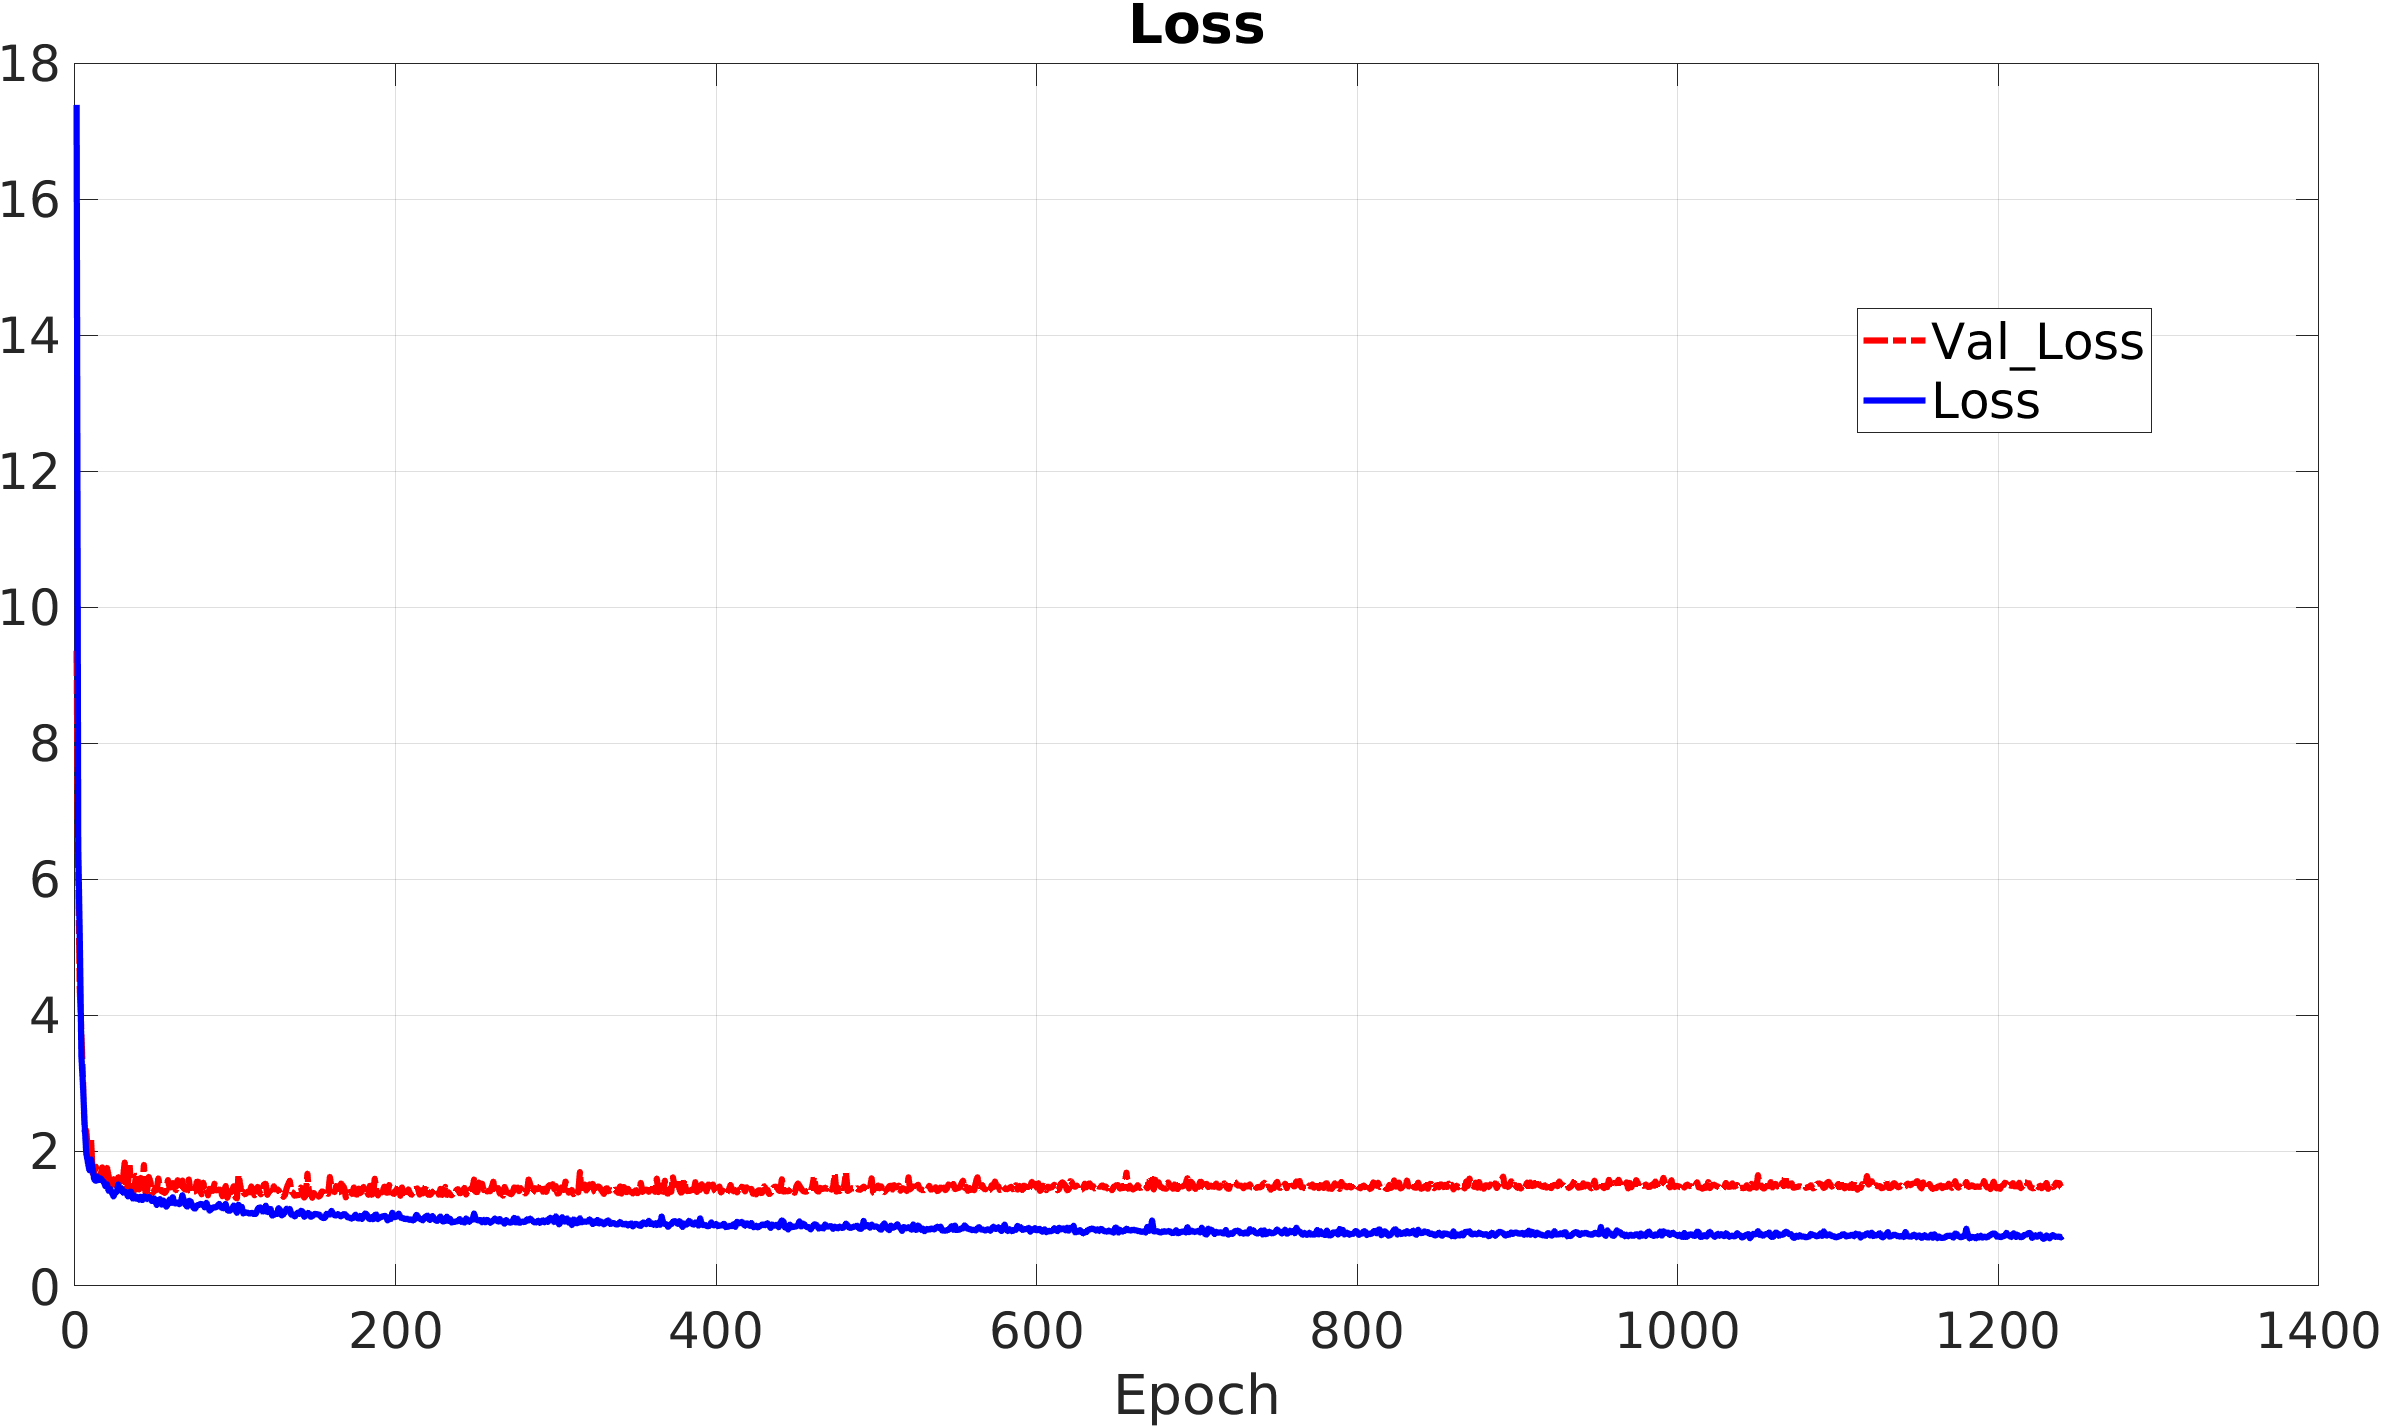
\includegraphics[width=\linewidth]{img/Cup_loss_noSmooth.png}
		\caption{MEE small mini-batch (32).}
		\label{img:smb}
	\end{minipage}
\end{figure}

\subsubsection{Explored hyper-parameters}
At the beginning, we ran grid search with large intervals and high steps. When we found the right interval we ran a grid search for each combination of the values:

\begin{itemize}
	\item Unit $\in$ \{25, 200\} with step $\in$ \{25, 50\};
	\item Learning rate $\in$ \{0.0001, 0.01\} with step $\in$ \{0.0001, 0.001\};
	\item Lambda $\in$ \{0, 0.004\} with step $\in$ \{0.0001,  0.0005\};
	\item Momentum $\in$ \{0, 0.8\} with step $\in$ \{0.05,  0.1\}.
\end{itemize}
\vspace{0.3cm}
We used the \texttt{tanh} activation function for all hidden layers and \texttt{linear} activation function in the output layer. We picked \texttt{tanh} because it gave the best result within all the other grid searches. \texttt{Linear} was chosen because it is often used as an output layer activation function for the regression problem.
For the training phase, we initialized the weight with a uniform distribution in the [-0.7, 0.7] interval.

\subsubsection{Grid search result}
Table \ref{tab:best_nets} reports the average of the values found for TR, VS and TS during the k-fold cross validation with k=3.   
\begin{center}
\small\addtolength{\tabcolsep}{-3pt}
\begin{table}[h!]
	\centering
	\begin{tabular}{|c|c|c|c|c|c|c|c|}
		\hline
		\textbf{Layer}& \textbf{Units}& \textbf{Learning rate} & \multicolumn{1}{l|}{\textbf{Lambda}} & \textbf{Momentum} & \textbf{Error TR}& \textbf{Error VS}& \textbf{Error TS}\\ \hline
			1 & 75 & 0.00450 & 0.00001 & 0.6  & 0.9676 & 1.1202 & 1.2151  \\
			1 & 100 & 0.00087 & 0.0000 & 0.8  & 0.9832 & 1.2750 &  1.2662\\
			1 & 100 & 0.00097 & 0.0000 & 0.8  & 0.9851 & 1.2759 &  1.2786\\
			1 & 100 & 0.00500 & 0.0000 & 0.5  & 0.9859 & 1.2845 & 1.2784 \\
			1 & 100 & 0.00500 & 0.0000 & 0.7  & 0.9752 & 1.2654 & 1.2569 \\
			1 & 100 & 0.00500 & 0.00001 & 0.6  & 0.8731& 1.2412 & 1.2375 \\
			2 & 150 & 0.00875 & 0.0002 & 0.8  & 0.8467 & 1.1332 &  1.1372 \\
			5 & 375 & 0.00450 & 0.0001 & 0.7  & 0.6323 & 1.1341 &  1.1341 \\
		  \hline
	\end{tabular}
		\caption{Best network configurations with MEE.}
		\label{tab:best_nets}
\end{table}
\end{center}
\newpage
The two models with more than one hidden layer have the following structure:
\begin{itemize}
	\item Two hidden layers: 100-50-2 (see fig. \ref{img::twolayer});
	\item Five hidden layers: 100-100-75-50-50-2 (see fig. \ref{img::fivelayer}).
\end{itemize}

\vspace{0.5cm}
\begin{figure}[H]
	\centering
	\begin{minipage}[t]{0.5\linewidth}
		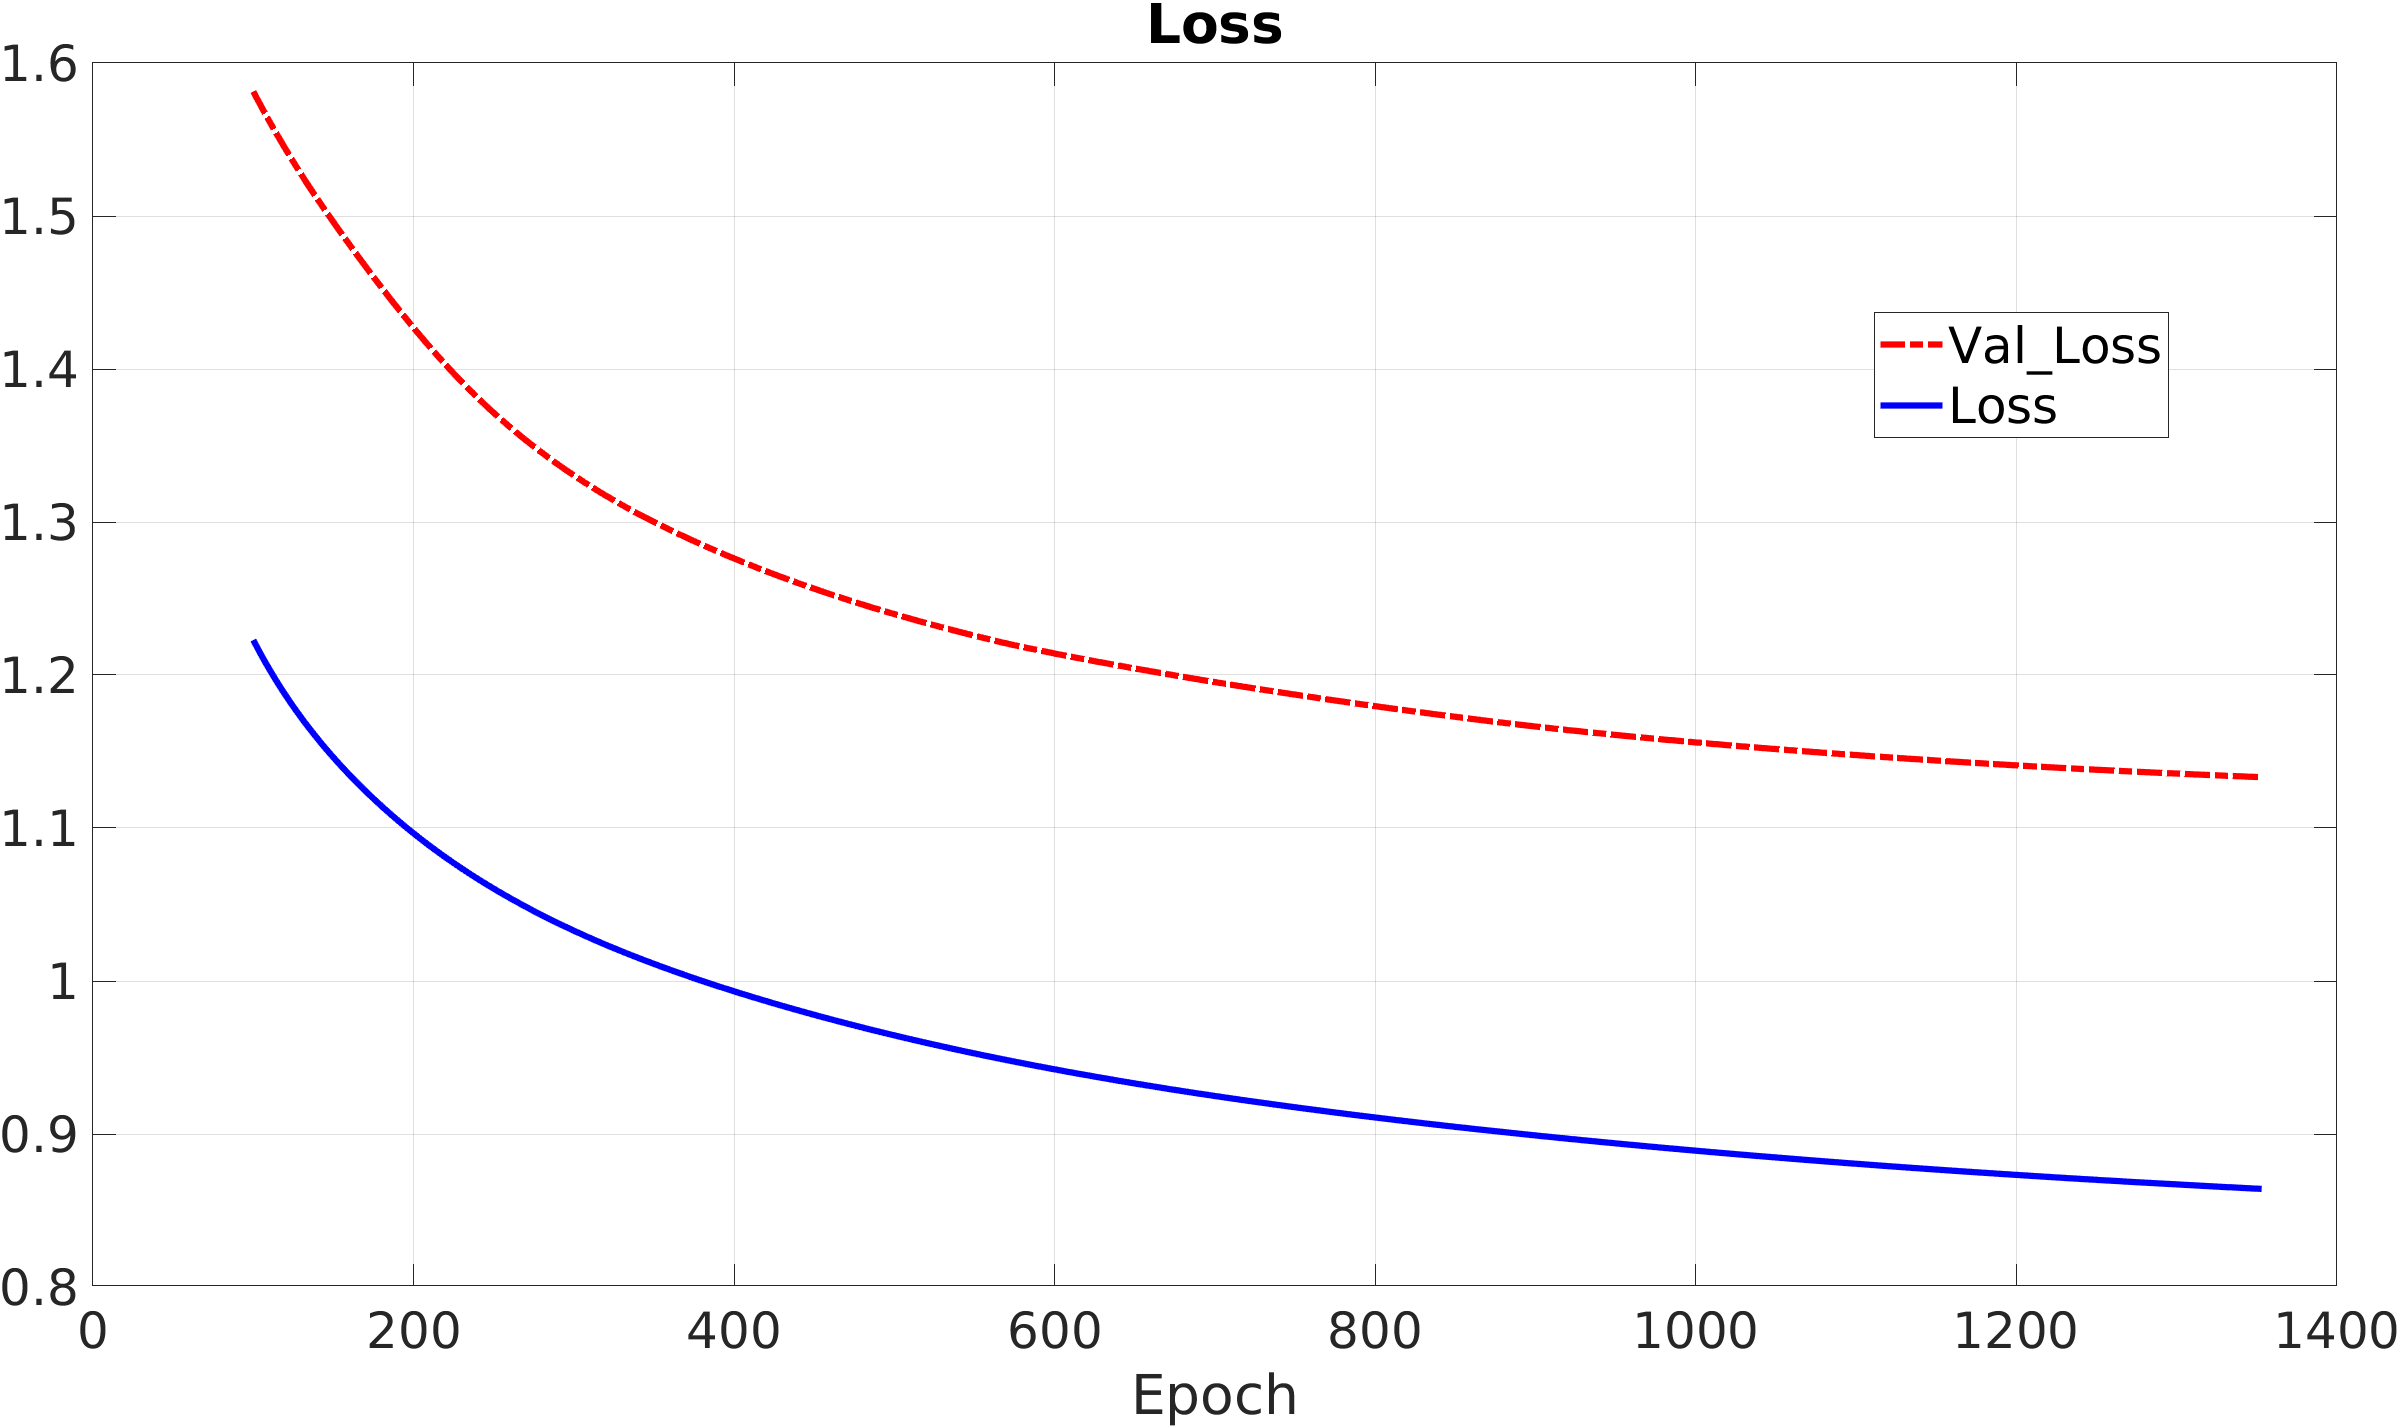
\includegraphics[width=\linewidth]{img/Cup_loss_Reg_Zoom_2l.png}
		\caption{MEE two hidden layer.}
		\label{img::twolayer}
	\end{minipage}%
	\begin{minipage}[t]{0.5\linewidth}
		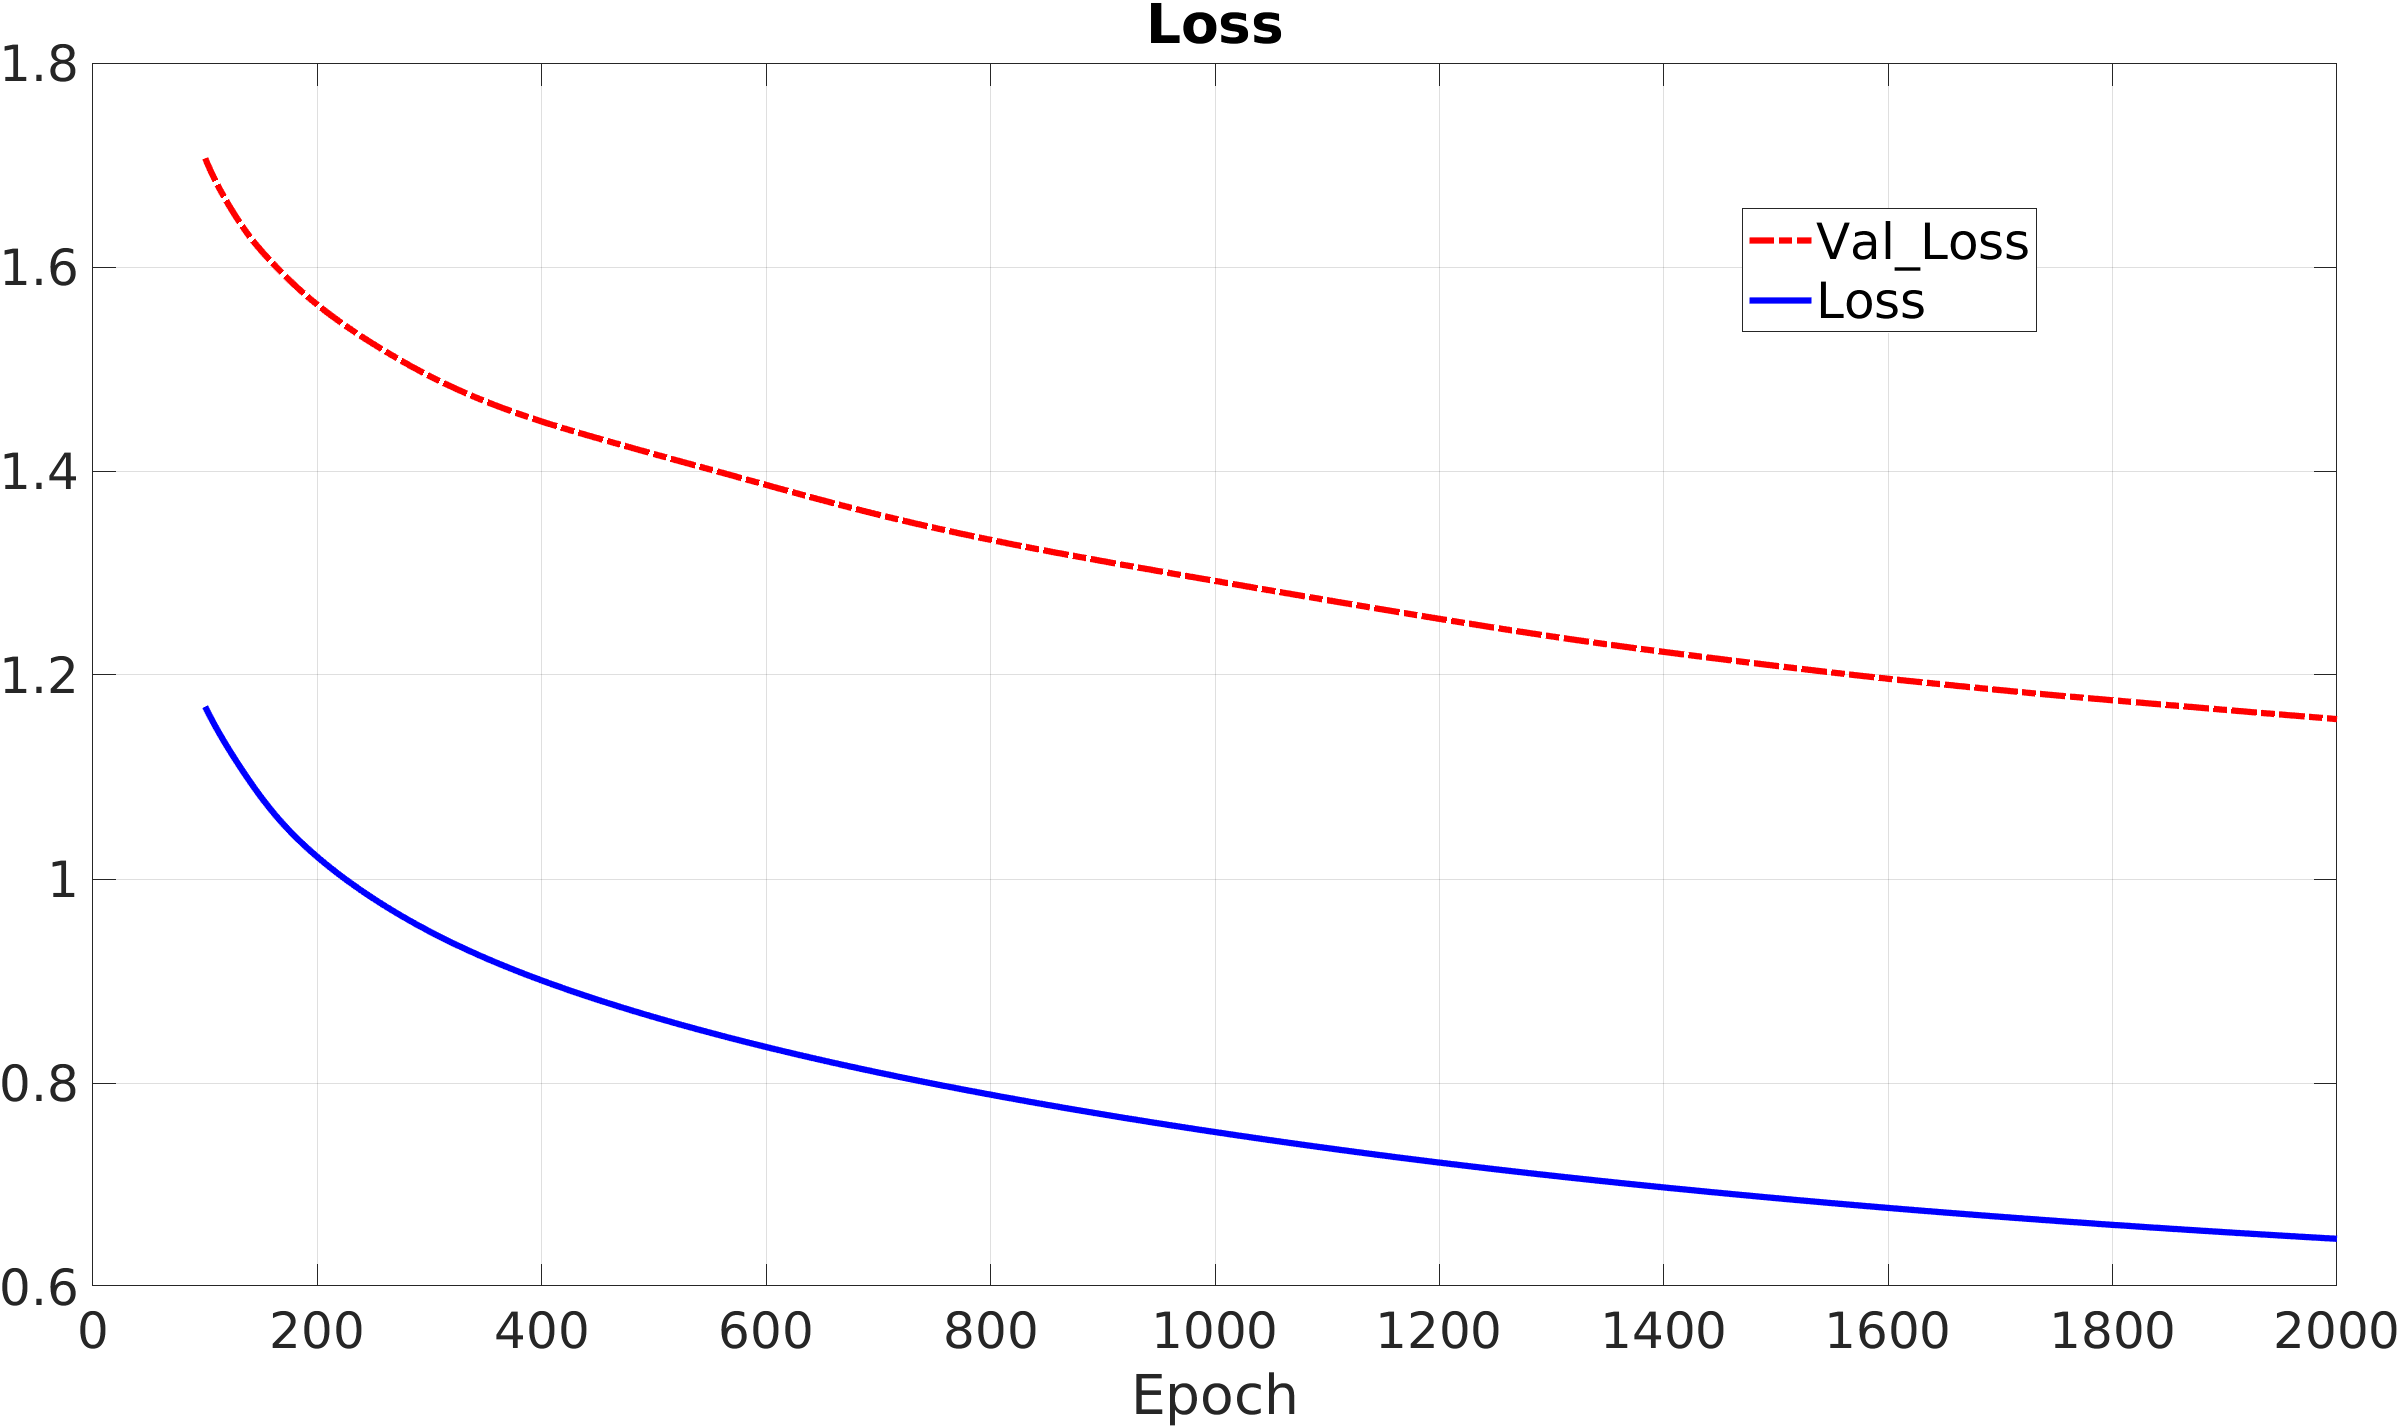
\includegraphics[width=\linewidth]{img/Cup_loss_Reg_Zoom_5l.png}
		\caption{MEE five hidden layer.}
		\label{img::fivelayer}
	\end{minipage}
\end{figure}

\subsubsection{Computing time}
We have developed a parallel grid search that allows us to take advantage of all our CPU cores automatically. All the computations were launched on the following machines:
\begin{itemize}
	\item Intel i7-8500Y, 1.5GHz;
	\item Intel i7-4720HQ, 2.6GHz.
	
\end{itemize}

The project was developed in C++ and the computational time and memory had to be strictly managed.
The time it takes to train on the MONK dataset with 800 epochs and 5 units is 1.5 seconds, for the ML CUP dataset with 8000 epochs and 75 units is 1.10 minutes.

\subsubsection{Comparisons}
We tried multiple neural networks with different number of layers and distinct types of gradient descent (stochastic, mini-batch and batch). We came to the conclusion that the number of layers does not significantly affect network generalization performance. Moreover with batch gradient descent we obtained the best learning curve.

\subsubsection{Chosen model}
The final model was chosen from the best models found after the grid search (table \ref{tab:best_nets}). It has the following hyper-parameters (table \ref{tab:best_net}) and MEE error for the training set, validation set and test set.
We achieved an average MEE of 1.2093 on our test set, taken as an average of seven
different trainings of the network (to avoid the bias due to the random weight
initialization).

\vspace{0.5cm}
\begin{center} 
\small\addtolength{\tabcolsep}{-3pt}
\begin{table}[h!]
	\centering
	\begin{tabular}{|c|c|c|c|c|c|c|c|}
		\hline
		\textbf{Layer}& \textbf{Units}& \textbf{Learning rate} & \multicolumn{1}{l|}{\textbf{Lambda}} & \textbf{Momentum} & \textbf{Error TR}& \textbf{Error VS}& \textbf{Error TS}\\ \hline
		1 & 75 & 0.00450 & 0.00001 & 0.6  & 0.9676 & 1.1202 & 1.2093  \\
		\hline
	\end{tabular}
	\caption{Best network configuration with MEE.}
	\label{tab:best_net}
\end{table}
\end{center}

We chose it because it was the model that performed better in the validation set. Also, its learning curve was smooth and stable.
The learning curve, also with an enlargement, is shown in figure \ref{img:best}.

\begin{figure}[H]
    \centering
    \begin{minipage}[t]{0.5\linewidth}
        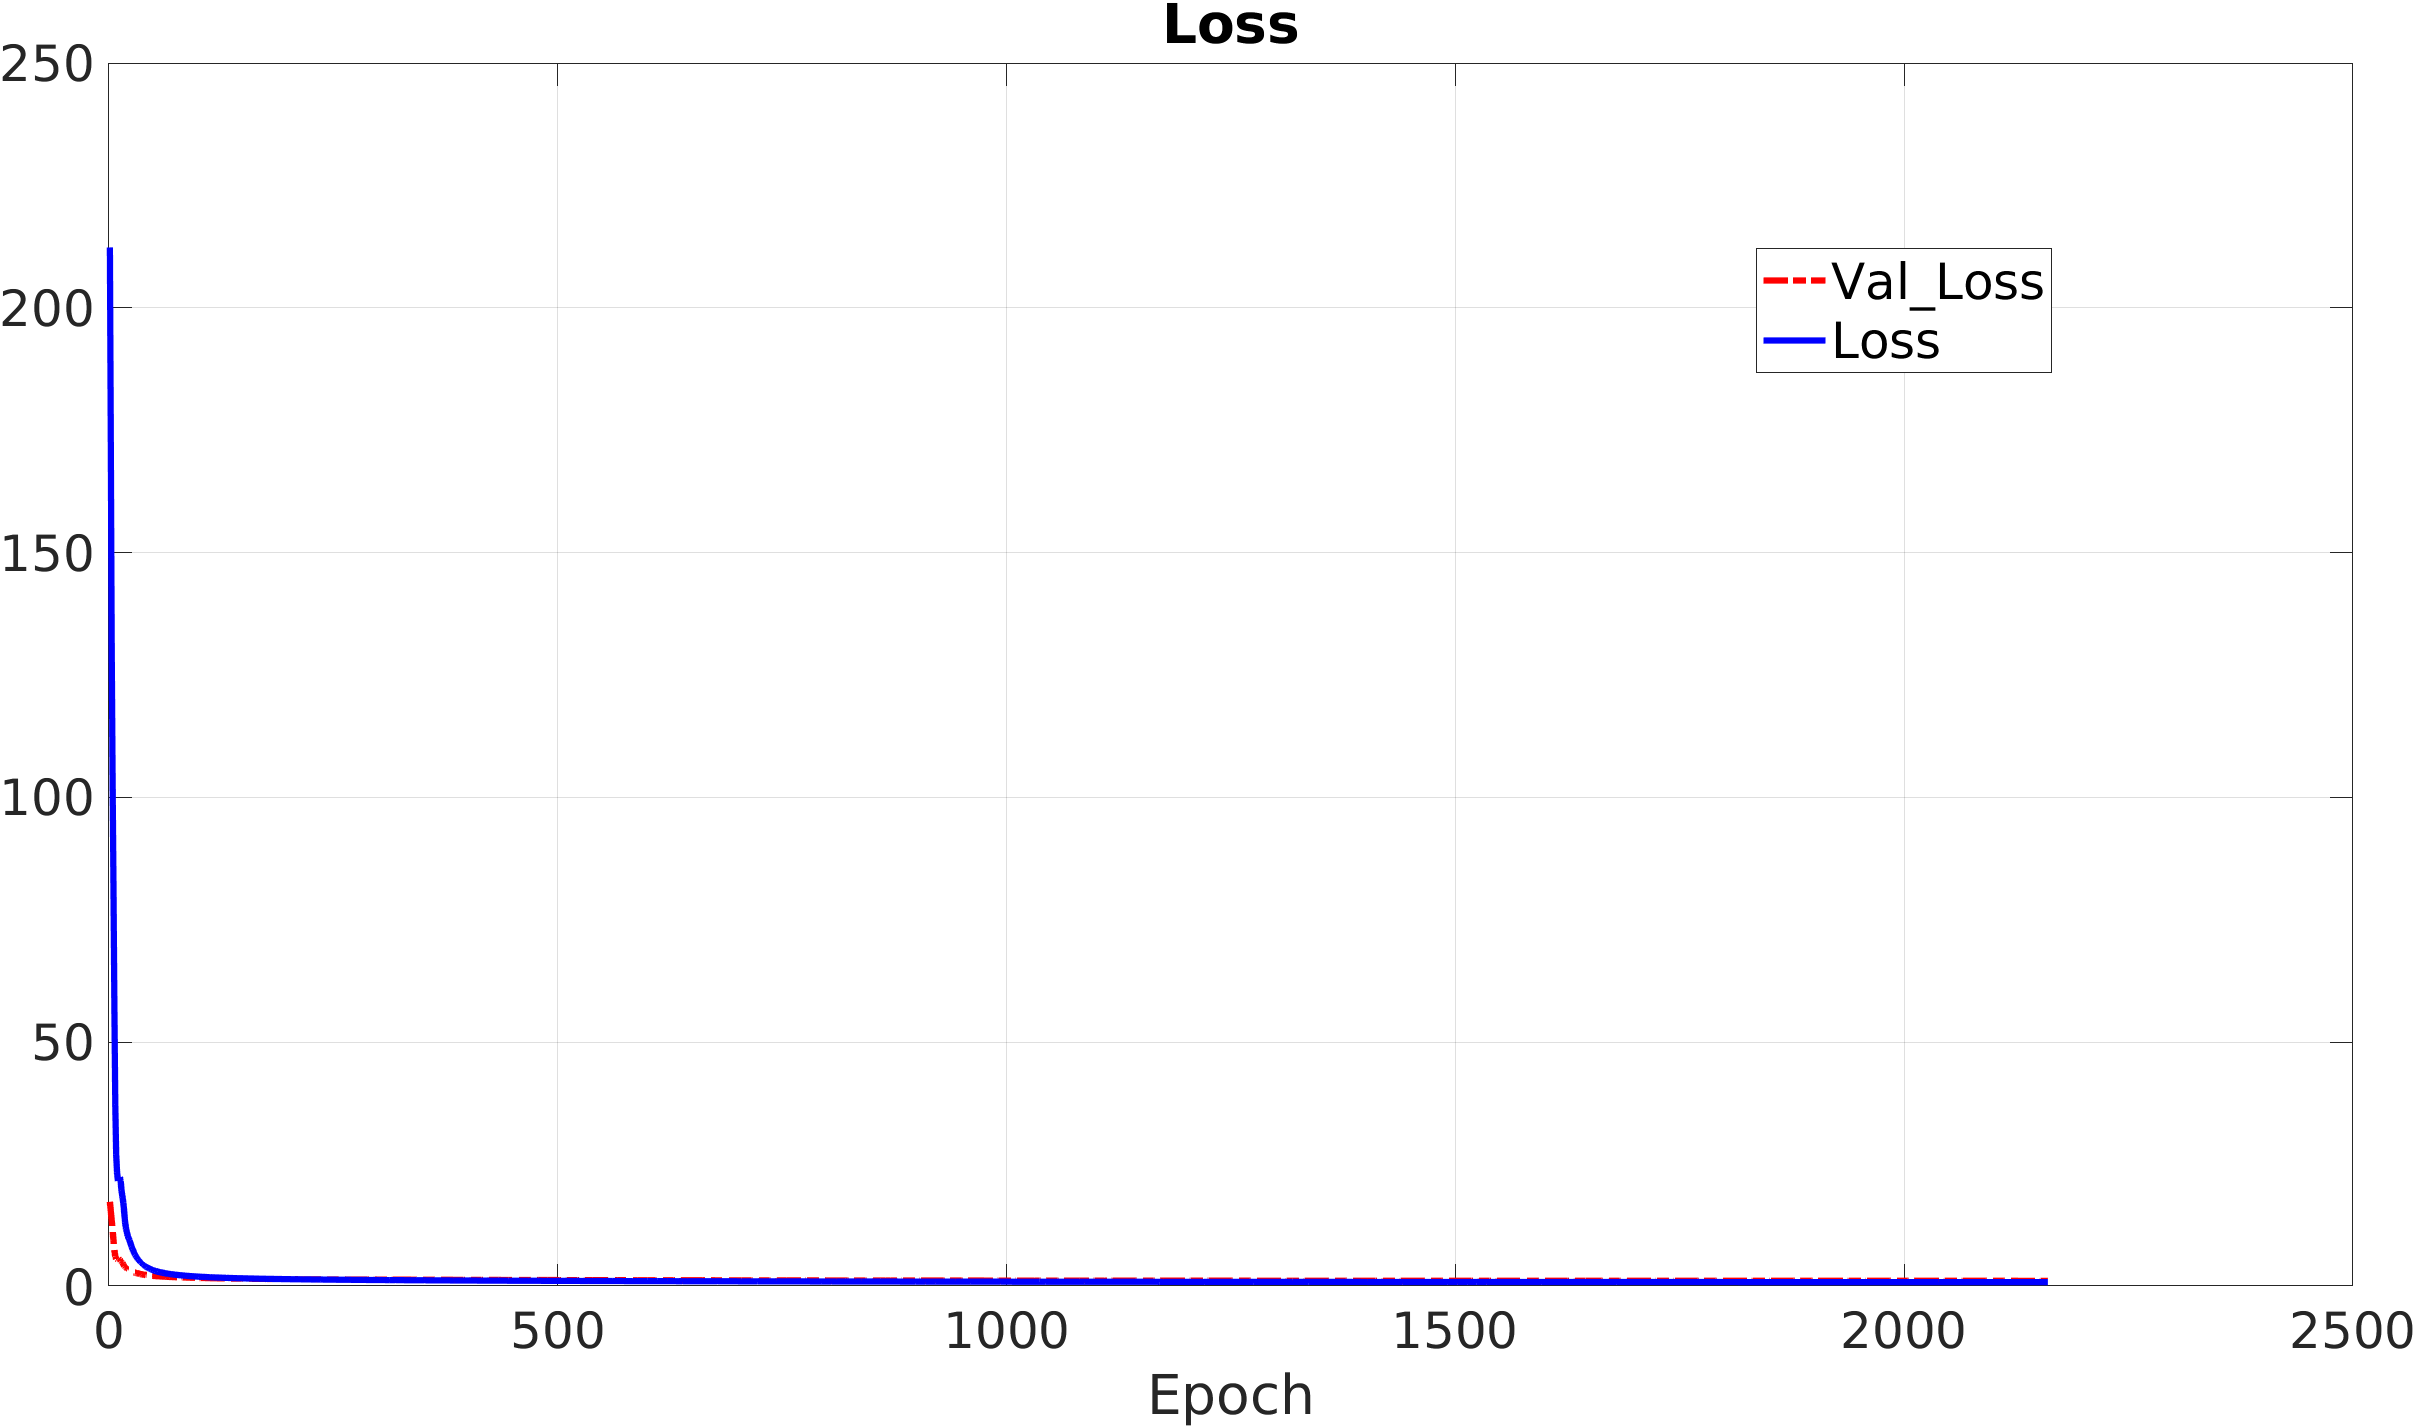
\includegraphics[width=\linewidth]{img/Cup_loss_Reg_noZoom.png}
        %\subcaption{MSE}
    \end{minipage}%
    \begin{minipage}[t]{0.5\linewidth}
        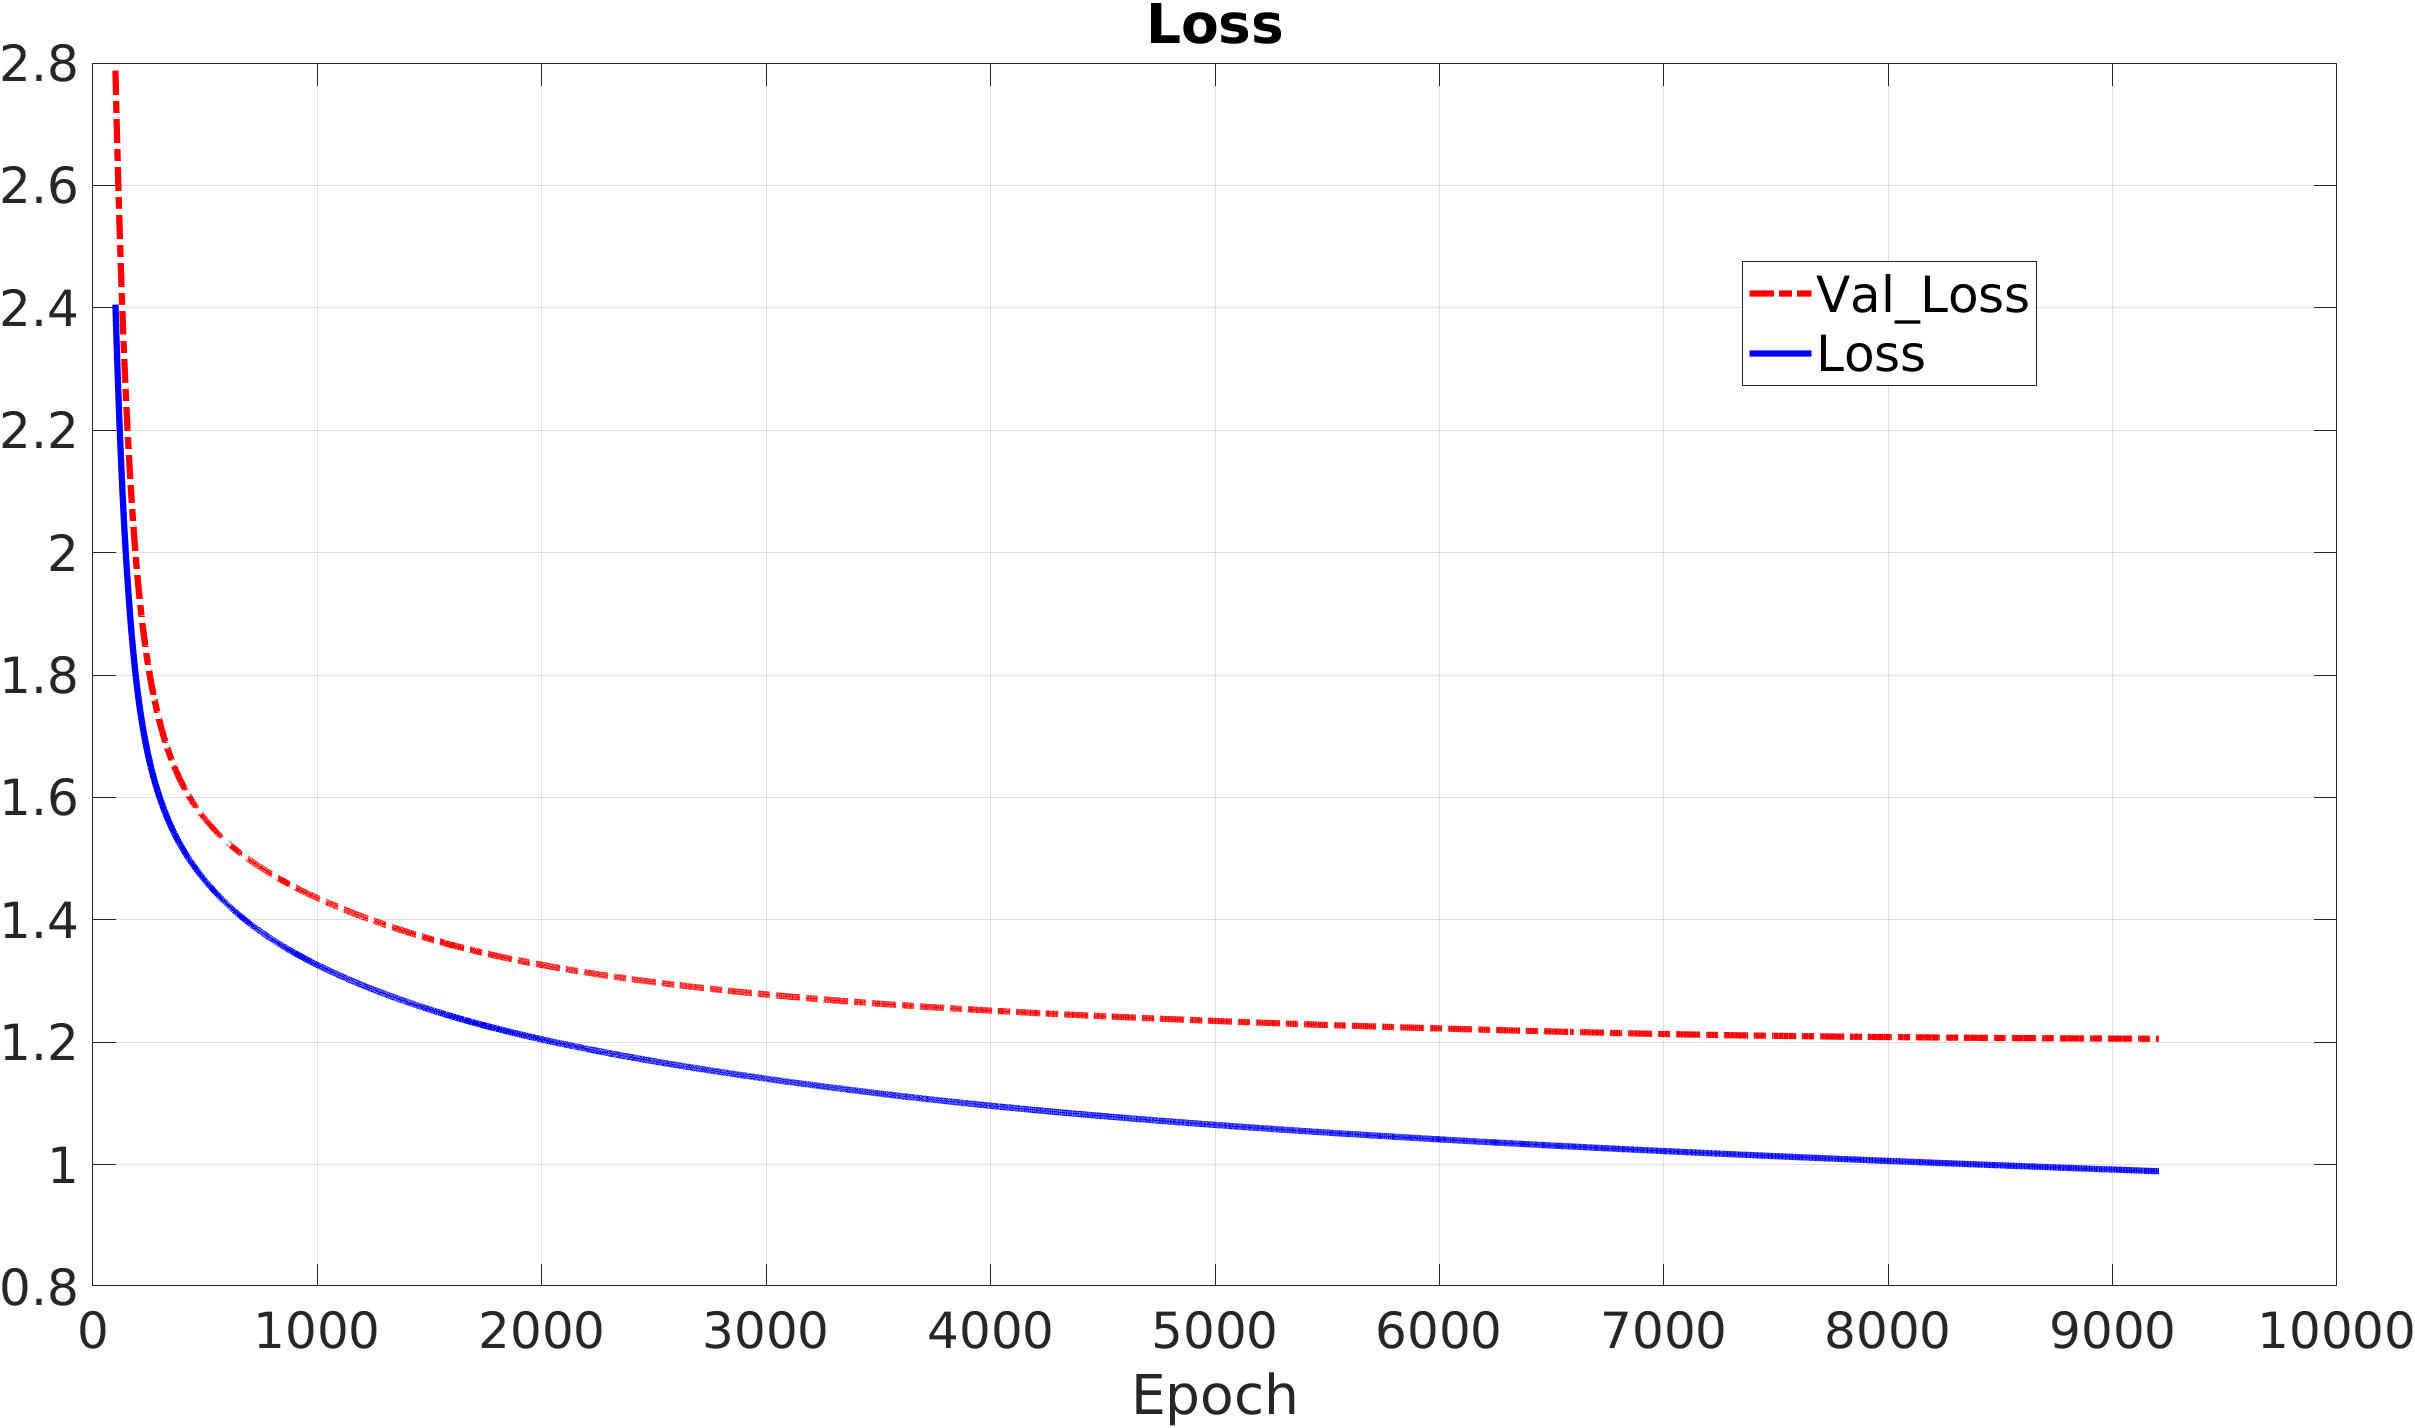
\includegraphics[width=\linewidth]{img/Cup_loss_Reg_Zoom.png}
        %\subcaption{Accuracy}
    \end{minipage}
    \caption{MEE and zoomed MEE for ML cup regularized.}
    \label{img:best}
\end{figure}



